\documentclass[envcountsect]{llncs}
\bibliographystyle{splncs04}
\pagestyle{headings}

% = = = = = Packages = = = = = %

% !TEX root = ../main.tex

%------------------------LNCS----------------------%

%None

%------------------------Packages----------------------%

% = = = Graphics
\usepackage[pdftex]{graphicx}
\graphicspath{{figures/}}
\DeclareGraphicsExtensions{.jpg,.png}
\usepackage[table,xcdraw]{xcolor}

% = = = Subfig (note not subfigure)
\usepackage[caption=false,font=footnotesize]{subfig}

% = = = Math Symbols
\usepackage{amsmath}
%\usepackage{amstext,amssymb,amsthm}
\usepackage{bbm}
\usepackage{stmaryrd}
\usepackage{wasysym}

\usepackage{color}
\usepackage{multirow}
\usepackage{rotating}
\usepackage{makecell}
\usepackage{hhline}
% = = = Other
\usepackage{array}
\usepackage{color}
\usepackage[hyphens]{url}
\usepackage[pdftitle=Title,pdfauthor=Anonymous]{hyperref}

%------------------------END----------------------%  
  


% !TEX root = ../main.tex
%------------------------Custom Commands----------------------%

% = = = Latin Short-forms (ie, eg, etc, et al)
\usepackage{xspace}
\newcommand{\etal}{\textit{et al.}\xspace}
\newcommand{\etc}{\textit{etc.}\xspace}
\newcommand{\ie}{\textit{i.e.,}\xspace}
\newcommand{\eg}{\textit{e.g.,}\xspace}
\newcommand{\cf}{\textit{cf.}\xspace}
\newcommand{\supra}{\textit{Supra}\xspace}
\newcommand{\nee}{\textit{n\'ee}\xspace}
\newcommand{\aka}{\textit{a.k.a.,}\xspace}



% = = = Arrow -> (\lt)
\newcommand{\lt}{$\rightarrow$\xspace}

% = = = Keywords (kw)
\newcommand{\kw}[1]{\textsf{#1}}

% = = = Colored text (textblue)
\newcommand{\textblue}[1]{\textcolor{blue}{#1}}

% = = = Compact Lists (compactlist, compactlistn)
\newenvironment{compactlist}
  {\begin{itemize} 
  \setlength{\itemsep}{0pt} 
  \setlength{\parskip}{0pt}} 
  {\end{itemize}}
  
\newenvironment{compactlistn}
  {\begin{enumerate} 
  \setlength{\itemsep}{0pt} 
  \setlength{\parskip}{0pt}} 
  {\end{enumerate}}
  
\renewcommand{\labelitemi}{$\bullet$}
  

%------------------------Crypto----------------------%  

% = = = Zp, Gq and Zq
\newcommand{\Zp}{\mathbb{Z}^{*}_{p}}
\newcommand{\Zq}{\mathbb{Z}_{q}}
\newcommand{\Gq}{\mathbb{G}_{q}}

% = = = Encryption, etc.
\newcommand{\Enc}[1]{\mathsf{Enc}(#1)}
\newcommand{\EncB}[1]{\llbracket #1 \rrbracket}
\newcommand{\ReRand}[1]{\mathsf{ReRand}(#1)}
\newcommand{\Hash}[1]{\mathcal{H}(#1)}
\newcommand{\Sign}[1]{\mathsf{Sig}(#1)}
\newcommand{\Comm}[1]{\mathsf{Comm}(#1)}
\newcommand{\Open}[1]{\mathsf{Open}(#1)}

% = = = Tuples
\newcommand{\tuple}[1]{\left \langle #1 \right \rangle}


%-------------------Custom for Paper----------------------%

% = = = Name
\newcommand{\Name}{\textsf{System Name}\xspace}
\newcommand{\dai}{\textsf{Dai}\xspace}
\newcommand{\cdp}{\textsf{CDP}\xspace}
\newcommand{\vault}{\textsf{Vault}\xspace}







% !TEX root = ../main.tex

\begin{table}[t!]
    \centering
    
        \begin{tabular}{lllllllllllllll}
    
    &
    \headrow{Can replace entire logic} &
    
    \headrow{can replace pre-specified part of logic} & 


    \headrow{Can replace entire state} &
    
    \headrow{can change pre-specified state variables} &
    
    \headrow{No need to deploy a new contract} &

    \headrow{No need to migrate state from old contract} &

    \headrow{No need to separate State and Logic} &

    \headrow{Function Selector Clashes Risk} &

    \headrow{Storage Clashes Risk} & 

    \headrow{No indirection} & 


    \headrow{User endpoint address not changed} &
    

    \headrow{Downtime in upgrade events} &

    \headrow{No need to change code to add the upgrade pattern} &

    \headrow{Need to change a state variable} 
    
    
    \\
    
    \hline
 
    
        \multicolumn{1}{c|}{Parameter change}	& \multicolumn{1}{c|}{}  & \multicolumn{1}{c|}{} &  \multicolumn{1}{c|}{} & \multicolumn{1}{c|}{\checkmark} & \multicolumn{1}{c|}{\checkmark} & \multicolumn{1}{c|}{\checkmark} &  \multicolumn{1}{c|}{\checkmark} &  \multicolumn{1}{c|}{} & \multicolumn{1}{c|}{} & \multicolumn{1}{c|}{\checkmark} & \multicolumn{1}{c|}{\checkmark} & \multicolumn{1}{c|}{} &\multicolumn{1}{c|}{\checkmark} & \multicolumn{1}{c}{\checkmark}\\
    
        \hline
  
        \multicolumn{1}{c|}{Component Change}	& \multicolumn{1}{c|}{}  & \multicolumn{1}{c|}{\checkmark} &  \multicolumn{1}{c|}{} & \multicolumn{1}{c|}{} & \multicolumn{1}{c|}{} & \multicolumn{1}{c|}{\checkmark} &  \multicolumn{1}{c|}{\checkmark} &  \multicolumn{1}{c|}{} &  \multicolumn{1}{c|}{} &  \multicolumn{1}{c|}{\XBox} & \multicolumn{1}{c|}{\checkmark} & \multicolumn{1}{c|}{} & \multicolumn{1}{c|}{\XBox} &  \multicolumn{1}{c}{\checkmark}\\
        

        \hline

        \makecell{Migration}	& \multicolumn{1}{|c|}{\checkmark}  & \multicolumn{1}{c|}{} &  \multicolumn{1}{c|}{\checkmark} & \multicolumn{1}{c|}{} & \multicolumn{1}{c|}{} & \multicolumn{1}{c|}{} &  \multicolumn{1}{c|}{\checkmark} &  \multicolumn{1}{c|}{} &  \multicolumn{1}{c|}{} &  \multicolumn{1}{c|}{\checkmark} & \multicolumn{1}{c|}{} & \multicolumn{1}{c|}{} & \multicolumn{1}{c|}{\checkmark} &  \multicolumn{1}{c}{}\\
    
         \hline


        \makecell{Call-based}	& \multicolumn{1}{|c|}{\checkmark}  & \multicolumn{1}{c|}{} &  \multicolumn{1}{c|}{} & \multicolumn{1}{c|}{} & \multicolumn{1}{c|}{} & \multicolumn{1}{c|}{\checkmark} &  \multicolumn{1}{c|}{} &  \multicolumn{1}{c|}{} &  \multicolumn{1}{c|}{} &  \multicolumn{1}{c|}{} & \multicolumn{1}{c|}{} & \multicolumn{1}{c|}{} & \multicolumn{1}{c|}{} & \multicolumn{1}{c}{\checkmark}\\
    
        \hline


        \makecell{DelegateCall-based}	& \multicolumn{1}{|c|}{\checkmark}  & \multicolumn{1}{c|}{} &  \multicolumn{1}{c|}{} & \multicolumn{1}{c|}{} & \multicolumn{1}{c|}{} & \multicolumn{1}{c|}{\checkmark} &  \multicolumn{1}{c|}{} &  \multicolumn{1}{c|}{\checkmark} & \multicolumn{1}{c|}{\checkmark}&  \multicolumn{1}{c|}{} & \multicolumn{1}{c|}{\checkmark} & \multicolumn{1}{c|}{} & \multicolumn{1}{c|}{\XBox} & \multicolumn{1}{c}{\checkmark}\\

        \hline

        \makecell{Diamonds}	& \multicolumn{1}{|c|}{\checkmark}  & \multicolumn{1}{c|}{} &  \multicolumn{1}{c|}{} & \multicolumn{1}{c|}{} & \multicolumn{1}{c|}{} & \multicolumn{1}{c|}{\checkmark} &  \multicolumn{1}{c|}{} &  \multicolumn{1}{c|}{\checkmark} & \multicolumn{1}{c|}{\checkmark\checkmark}&  \multicolumn{1}{c|}{} & \multicolumn{1}{c|}{\checkmark} & \multicolumn{1}{c|}{} & \multicolumn{1}{c|}{\XBox} & \multicolumn{1}{c}{\checkmark}\\
        
        
         \hline

        \makecell{Metamorphic}	& \multicolumn{1}{|c|}{\checkmark}  & \multicolumn{1}{c|}{} &  \multicolumn{1}{c|}{\checkmark} & \multicolumn{1}{c|}{} & \multicolumn{1}{c|}{} & \multicolumn{1}{c|}{} &  \multicolumn{1}{c|}{\checkmark} &  \multicolumn{1}{c|}{} & \multicolumn{1}{c|}{}&  \multicolumn{1}{c|}{\checkmark} & \multicolumn{1}{c|}{\checkmark} & \multicolumn{1}{c|}{\checkmark} & \multicolumn{1}{c|}{\checkmark} &  \multicolumn{1}{c}{}\\
        
        
         \hline
        
        
        \end{tabular}
        \captionsetup[tabular]{singlelinecheck=off}
        \caption{Evaluation}
       
    
    \end{table}
    \footnotetext[1]{Design of system in which a parameter can change the logic is hard}

%\usepackage[all=normal,floats=tight,paragraphs=tight]{savetrees}
\usepackage{fullpage}

% = = = = = Title = = = = = %

\begin{document}
\frontmatter
\mainmatter

\title{Not so immutable: Upgradeability of Smart Contacts on Ethereum}
\author{Mehdi Salehi\inst{1} \and Jeremy Clark\inst{1} \and Mohammad Mannan\inst{1}}
\institute{Concordia University, Montreal, Canada}

\maketitle


% = = = = = Abstract = = = = = %

% !TEX root = ../main.tex

\begin{abstract}
A smart contract that is deployed to a blockchain system like Ethereum is, under reasonable circumstances, expected to be immutable and tamper-proof. This is both a feature (promoting integrity and transparency) and a bug (preventing security patches and feature updates). Modern smart contracts use software tricks to enable upgradability, raising the research questions of \textit{how} upgradeability is achieved and \textit{who} is authorized to make changes. In this paper, we summerize and evaluate six upgradability patterns. We develop a measurement framework for finding how many upgradeable contracts are on Ethereum that use certain prominent upgrade patters. We also measure how they implement access control over their upgradability: about 50\% are are controlled by a single Externally Owned Address (EOA), and about 20\% are controlled by multi-signature wallets in which a limited number of persons can change the whole logic of the contract.

%% Smart contracts are peices of codes that are deployed to the blockchain systems, to remove the barrier of trusting middleman to run specific logic. Ethereum is the first and mostly used public blockchain that introduced rich smart contracts that are not just limited to some specific scripts (like Bitcoin scripting language). Smart contracts are supposed to be immutable and tamper proof which means the code cannot be changed just after deployment to the blockchain. This feature of smart contracts are in contrast with Software Engineering idealogy, because codes are prone to bugs and also new features and functionalities need to be added to the software.
%% During the time, huge hacks happened to Ethereum smart contracts (e.g. DAO hack) which brought developers to rethink about the immutability and find ways to change the smart contracts after deployment to the blockchain. Two main questions in this regard is \textit{how to add upgradeability to the smart contract?} and \textit{who is responsible to enforce changes to the system?}.

%% In this paper we explore how developers torture an immutable blockchain into allowing smart contracts to be upgraded. To answer the first question we investigate all different patterns in the wild that bring upgradeability feature to Ethereum smart contracts. Then we evaluate each pattern to give developers insight that which pattern is proper for their Decentralized Application (Dapp) and the pros and cons of each pattern. The most used upgradeability pattern in Ethereum blockchain right now is called \textbf{Proxy Patterns}.
%% In the later part of the paper we proposed a novel way to find smart contracts that use Proxy Patterns to add upgradeability feature by investigating all transactions confirmed to the Ethereum blockchain for a period of one year starting from September 2020. 

%% To answer the second question we examine all proxy contracts we have collected from the previous analysis, to find their \textit{admin account}, the agent authorized to upgrade the system, and find their admin type; Externlly Owned address (EOA) in which one person can decide to change the system, Multi-Signature Wallets in which limited number of persons can change the system and Decentralized Governance models. The first two admin types are bring risks to the system and these are against the sprit of decentralization in blockchain space. 

\end{abstract}

% = = = = = Main Body = = = = = %

% !TEX root = ../main.tex

% = = = = = = = = = = = = = = = = = = = = = = = = = = = = = = = = = = = = = = = = = =

\section{Introductory Remarks}

The key promise of a smart contract running on Ethereum is that its code will execute exactly as it is written, and the code that is written can never be changed. While Ethereum cannot maintain this promise unconditionally, its assumptions (\eg cryptographic primitives are secure and well-intentioned participants outweigh malicious ones) provide a realistic level of assurance. 

The immutability of a smart contract's code is related to trust. If Alice can validate the code of a contract, she can trust her money to it and not be surprised by its behaviour. Unfortunately, disguising malicious behaviour in innocuous-looking code is possible (`rug pulls'), and many blockchain users have been victims. On the other hand, if the smart contract is long-standing with lots of attention, and security assessments from third-party professional auditors, the immutability of the code can add confidence. 

The flip-side of immutability is that it prevents software updates. Consider the case where a security vulnerability in the code of a smart contract is discovered. Less urgently, some software projects may want to roll out new features, which is also blocked by immutability. There is an intense debate about whether this is a positive or negative, with many claiming that `upgradability is a bug.' We do not take a position on this debate. We note that upgradability is happening and we seek to study what is already being done and what is possible. 

Is there a way to deploy upgradeable smart contracts if all smart contracts are (practically speaking) immutable? Consider a two simple ideas. The first is to deploy the upgraded smart contract at a new address. One main drawback to this is that all software and websites need to update their addresses. A second simple idea is to use a proxy contract (call it P) that stores the address of the `real' contract (call it A). Users consider the system to deployed at P (and might not even be aware it is proxy). When a function is called on P, it is forwarded to A. When an upgrade is deployed to a new address (call it B), the address in P is changed from A to B. This solution also has drawbacks. For example, if the proxy contract hardcodes the list of functions that might be called on A, new functions cannot be added to B. Another issue is that the data (contract state) is stored in A. For most applications, a snapshot of A's state will need to be copied to B without creating race conditions. Mitigating these issues leads to more elaborate solutions like splitting up a contract logic and state, utilizing Ethereum-specific tricks (fallback functions to capture unexpected function names), and trying to reduce the gas costs of indirection between contracts.

\paragraph{Contributions.} 

\textblue{Finalize this text later.} %In the following sections we classify different ways of upgradeability on Ethereum blockchain, and describe pros and cons of each approach. Then we evaluate the upgradeability methods and compare them with each other. We conducted a measurement study in the most favorable upgrade pattern in Ethereum blockchain and give a dataset of them. Also we will talk about possible agents that is responsible for the changes on the Dapps. In the last part we will talk about some problems we are facing in the upgrade process and the ways that we can handle them.

% = = = = = = = = = = = = = = = = = = = = = = = = = = = = = = = = = = = = = = = = = =

\section{Background and Related Work}

%\begin{figure}[t]
%  \centering
%      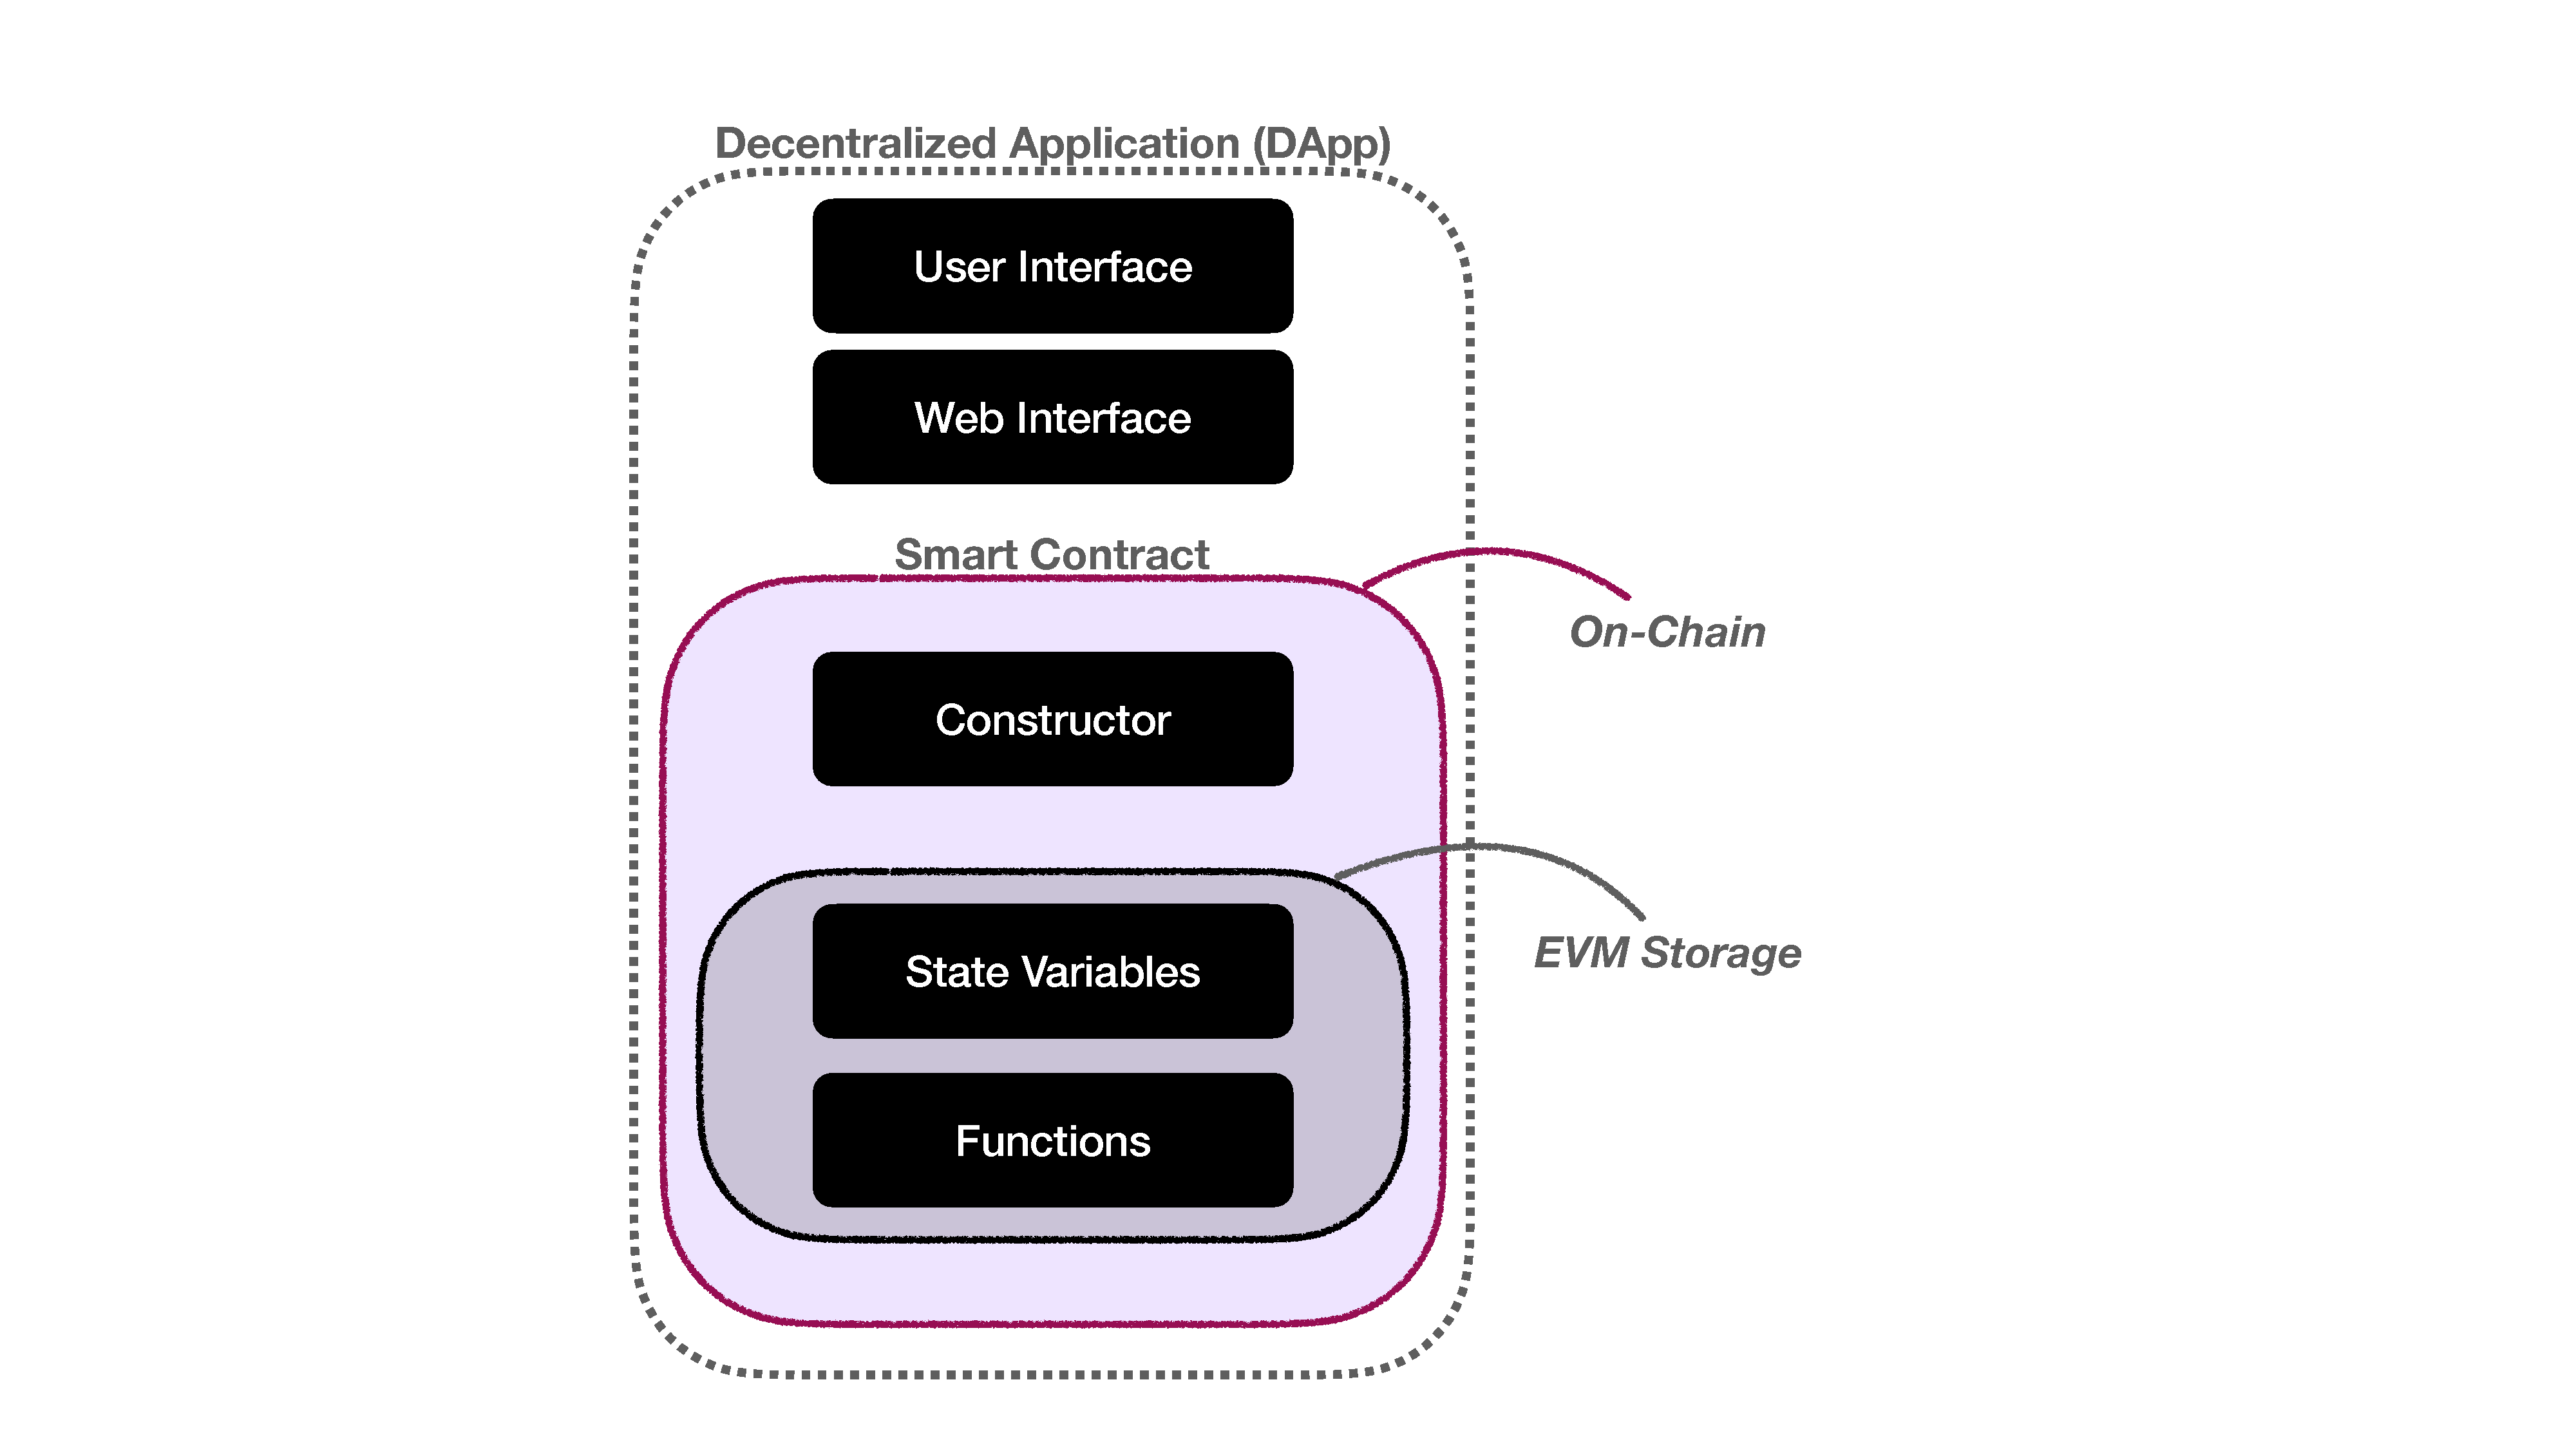
\includegraphics[width=0.4\textwidth]{figures/dapp.pdf}
%  \caption{Components of a decentralized application.\label{fig:dapp}}
% \end{figure}

%\paragraph{DApp vs. smart contract.} Figure~\ref{fig:dapp} shows the main components of a decentralized application (DApp). The core component is the smart contract (or simply contract), which is the set of functions and state stored on-chain. When first deployed, the smart contract also includes a constructor function which executes once and is then discarded (to be more precise, a copy of the constructor is stored in the record of transactions, called the calldata, but it is not retained in the EVM and can never be called again). While it is possible to interact directly with a smart contract by invoking its functions through Ethereum, generally users are provided an off-chain website with a user interface. Website actions are translated into calls to the Ethereum network through a set of tools (most prominently web3) in the web interface. 

\paragraph{Updating vs. upgrading.} Software maintenance is part of software's lifecycle, and the process of changing the product after delivery. Often a distinction is drawn between software \textit{updates} and software \textit{upgrades}. An update modifies isolated portions of the software to fix bugs and vulnerabilities. An upgrade is generally a larger overhaul of the software with significant changes to features and capabilities. In our paper, we will only use the term upgrade and instead distinguish between retail (parameters and isolated code) and wholesale (entire application) changes to a smart contract. While upgrades to a smart contract's user interface (UI) can significantly change a user experience and expose new features, UIs are governed by traditional software maintenance. Our paper only considers the on-chain smart contract component, which is significantly more challenging to upgrade as it is on-chain and immutable under reasonable circumstances. 

\paragraph{Related work.} 

A lot has been written in the non-academic arena as technical blog posts ~\cite{}. MOst of section 3 is based on this information. 

CREATE2 paper -> Measurements for only Metamoprhis, we do mostly proxy. ``Using simple heuristics derived from the EIPS we found 223,873 following EIP-897, 0 following EIP-1167, 22,238 following EIP-1822, and 31,432 following EIP-1967.'' By comparison, our model is more generic. 

USENIX paper -> tool for actually updating a contract, assuming the contract uses a delegatecall-based data seperation pattern. 
``Dissimilar Redundancy in DeFi'' -> another tool. 

Other researchers have measurement studies on Ethereum data but concern other aspects: tokens (two erc20), volnerabilities (10 papers), cost of opcodes, impacts of EIP-1559, xxx.

SELFDISTRUCT survey -> contract migration, clean up the old contract. Also useful for metamoprhisis but authors don't cover this

* we are measurement
* no tools
* broad set of upgrade pattern


\textblue{TBD}

% = = = = = = = = = = = = = = = = = = = = = = = = = = = = = = = = = = = = = = = = = =

\section{Classification of Upgrade Patterns}

\begin{figure}[t]
  \centering
      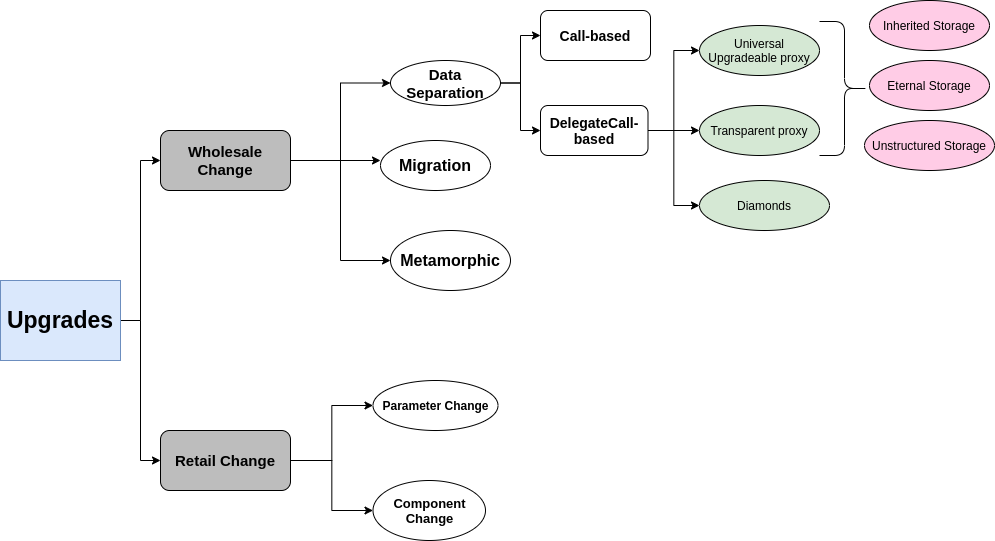
\includegraphics[width=0.8\textwidth]{figures/New_Classification.png}
  \caption{Classification. \textblue{Re-arrange to match ordering of text. Include section numbers of leaf nodes.}\label{fig:class}}
 \end{figure}
 
A variety of upgradeability patterns have been proposed for smart contracts. Most leverage Ethereum-specific operations and memory layouts and are not applicable to other blockchain systems.

% Misc notes:
% We have some off-chain upgrades like what people did to force UNISwap using arbitrum as the L2 solution. It is an off-chain upgrade not an automated one.
% Does Factory patterns can be defined as upgradeability patterns? Like creating a new pool for Uniswap!


% JC: It seems the evaluation table will capture this. Plus are these pros/cons relative to each other or to other kinds of upgradeability (assuming the latter, it is hard to discuss until we have shown how they work). 
%The \textit{Pros and Cons} for retail changes methods are:
%\begin{itemize}
%  \item Pros
%  \begin{itemize}
%    \item Simple to implement
%    \item Easy to audit
%  \end{itemize}
%  \item Cons
%  \begin{itemize}
%    \item Cannot fix a bug
%    \item Cannot add/change Logic in Parameter Configuration
%    \item Cannot add new Logic in Tweak Strategy
%  \end{itemize}
%\end{itemize}

% = = =

\subsection{Parameter Configuration}
\label{sec:parameter}

We first categorize upgradeability patterns into two main classes: \textit{retail changes} and \textit{wholesale changes}. A pattern for retail change does not enable the replacement of the entire contract. Rather, a component of the contract is pre-determined (before the contract is deployed on Ethereum) to allow future upgrades, and the code is adjusted to allow these changes. 

The simplest upgrade pattern is to allow a system parameter, that is stored in a state variable, to be changed. This requires a \textit{setter function} to overwrite (or otherwise adjust) the variable, and access control over who can invoke the function. For example, in decentralized finance (DeFi), many services have parameters that control fees, interest rates, liquidation levels, \etc. Adjustments to these parameters can initiate large changes in how the service is used (its `tokenomics'). A DeFi provider can retain control over these parameters, democratize control to a set of token holders (\eg stability fees in the stablecoin project MakerDao), or lock the parameters from anyone's control. In Section~\ref{sec:governance}, we dive deeper into the question who can upgrade a contract. 

% = = =

\subsection{Functional Component Change}
\label{sec:component}

While a parameter change allows an authorized user to overwrite memory, a functional component change addresses modifications to the code of a function (and thus, the logic of the contract). In the EVM, code cannot be modified once written and so new code must be deployed to a new contract, but can be arranged to be called from the original contract. 

One way to allow upgradable functions is deploying a helper contract that contains the code for the functions to be upgradeable. Users are given the address of the primary contract, and the address of this secondary (helper) contract is stored as a variable in the primary contract. Whenever thhis function is invoked at the primary contract, the primary contract is pre-programmed to forward the function call, using the opcode \texttt{Call}, to the address it has stored for the secondary contract. To modify the logic of the function, a new secondary contract is deployed at a new address, and an authorized set of individuals can then use a parameter change in the primary contract to update the address of the secondary contract.

The DeFi lending platform Compound uses this pattern for their interest rate models which are tailored specifically for each asset. The model for one asset can be changed without impacting the rest of the contract.

Upgradeable functional components need to be pre-determined before deploying the primary contract. Once the primary contract is deployed, it is not possible to add upgradeability to existing (non-upgradable) functions. It also cannot be directly used to add new functions to a contract. Finally, this pattern is most straightforward when the primary contract only uses the return value from the function to modify its own state. Thus, the function is either `pure' (relies only on the parameters to determine the output) or `view' (can read state from itself or other contracts, but cannot write state). If the function modifies the state of the primary contract, the primary contract must either expose its state variables to the secondary contract (by implementing setter functions), or it can run the function using \texttt{DelgateCall} if the secondary contract has no state of its own. 

This upgrade pattern suggests a way forward for wholesale changes to the entire contract: create a generic `proxy' contract that forwards all functions to a secondary contract. To work seamlessly, this requires some further engineering (sections~\ref{sec:callbased} and \ref{sec:delegatecall}).

% = = =

% \paragraph{Pluggable Modules}. In this pattern we have a core contract that have some immutable features and then new contracts generated by the main contract and each have some or all features of the main contract. This pattern is mostly used in wallets and DeFi services like DeFi saver and InstaDapp. Users can decide to add new features into their wallet. 


%We need upgradeability to fix a bug or adding a new feature. In the event of fixing a bug, the agent who is responsible for the upgrade need to be as quick as possible to address a security issue or bug and so there is no need to have consensus of the users of the Dapp to make change. But, in the latter case the agent must get the consensus of the Dapp users to change and add a new feature, so they do not need to be quick. This fact is another paradox in the upgradeability of smart contracts because these two different events are not distinguishable before occurring and so we cannot implement two different ways of upgrading a system (one for resolving bug, and one for adding feature). So, as a system designer, if decide to add upgradeability feature should select one of these as the main goal of adding upgradeability and design the system based on that.

% = = =

\subsection{Consensus Override}
\label{sec:hardfork}

The two previous patterns enable portions of a smart contract to be modified. The remaining patterns strive to allow an entire contract to be modified or, more simply, replaced. The first wholesale pattern is not a tenable solution to upgradeability as it as only been used rarely under extraordinary circumstances, but we include it for completeness. 

Immutability is enforced by the consensus of the blockchain network. If participating nodes (\eg miners) agreed to suspend immutability, they can in theory allow changes to a contract's logic and/or state. If agreement is not unanimous, the blockchain can be forked into two systems---one with the change and one without. In 2016, a significant security breach of a decentralized application called `the DAO' caused the Ethereum Foundation to propose overriding the immutability of this particular smart contract to reverse the impacts of attack. In the unusual circumstances of this case, it was possible to propose and deploy the fix before the stolen ETH could be extracted from the contract and circulated. Nodes with a philosophical objection to overriding immutability continued operating, without deploying the fix, under the name Ethereum Classic.
%Need to talk about L2 (Roll-ups) --> They can roll-back the chain state similar to the DAO fork (they can setup new desired rollup state and bridge regarding that).
%\textbf{Upgradeability is a Bug!}~\cite{Upg-Bug}.


% = = =

\subsection{Contract Migration}
\label{sec:migration}

The simplest wholesale upgrade pattern is to deploy a new version of the contract at a new address, and then inform users (and the web applications they use) to use the new version---called a `social upgrade.' One example is Uniswap, which is on version 3 at the time of writing. Versions 1 and 2 are still operable at their original addresses. 

Contract migration does not require developers to instrument their contracts with any new logic to support upgradability, as in many of the remaining patterns, which can ease auditability and gas costs for using the contract. However for most applications, there will be a need to transfer the data stored in the old contract to the new version. This is generally done in one of two ways. The first is to collate the state of the old contract off-chain and load it into the new contract (\eg via its constructor). If the old contract was instrumented with an ability to pause it, this can eliminate race-conditions that could otherwise be problematic during the data migration phase. The second method, specific to certain applications like tracking a user's balance of tokens, is to have the user initiate (and pay the gas) for a transfer of their balance from the old system to the new one.
 
 % JC: do we *need* one or it is useful?
 %Also we need a \textit{Migrator} contract if we decided to outsource the data migration into the users.
 
 % = = =

\subsection{\texttt{CREATE2}-based Metamorphosis}
\label{sec:metamorphic}

Is it possible to do contract migration, but deploy the new contract to the \textit{same} address as the original contract, effectively overwriting it? If so, developers can dispense with the need for a social upgrade (but would still need to accomplish data migration). At first glance, this should not be possible on Ethereum, however a set of opcodes can be `abused' to allow it: specifically, the controversial\footnote{\href{https://www.reddit.com/r/ethereum/comments/lx32kv/expectations\_for\_backwardsincompatible\_changes/}{``Expectations for backwards-incompatible changes / removal of features that may come soon.'' V. Buterin, Reddit r/ethereum, Mar 2021.}} \texttt{SELFDESTRUCT} opcode and the 2019-deployed \texttt{CREATE2}. 

Consider a contract, called Factory, that has the bytecode of another contract, A, that Factory wants to deploy at A's own address. \texttt{CREATE2}, which supplements the original opcode \texttt{CREATE}, provides the ability for Factory to do this and know in advance what address will be assigned to contract A, invariant to when and how many other contracts that Factory might deploy.  The address is a structured hash of A's ``initialization'' bytecode, parameters passed to this code, the factory contract's address, and a salt value chosen by the factory contract.\footnote{Specifically: $\mathsf{addr} \leftarrow \mathcal{H}(\mathtt{0xff} \| \mathsf{factoryAddr} \| \mathsf{salt} \| \mathcal{H} (\mathsf{initBytecode} \| \mathsf{initBytecodeParams}))$} Most often, A's initialization bytecode contains a copy of A's actual code (``runtime'' bytecode) to be stored on the EVM, and the initialization code is prepended with a simple routine to copy the runtime code from the transaction data (calldata) into memory and return. Importantly, however, the initialization bytecode might not contain A's runtime bytecode at all, as long as it is able to fetch a copy of it from some location on the blockchain and load it into memory. In order for \texttt{CREATE2} to complete, the address must be empty, which means either (1) no contract has ever been deployed there, or (2) a contract was deployed but invoked \texttt{SELFDESTRUCT}.

%It is also common that A's initialization code will initialize some of A's storage variables (\eg the code specified in the constructor function in Solidity) using parameters passed into it. 

%The initialization bytecode passed to \texttt{CREATE2} will be recorded in the transaction call and then executed, but it is not stored in contract A. The expected result of executing the initialization bytecode is that contract A's runtime bytecode will be deployed at the determined address. 

Assume the developer wants to deploy contract A using metamorphosis and later update it to contract B.\footnote{\href{https://medium.com/@0age/the-promise-and-the-peril-of-metamorphic-contracts-9eb8b8413c5e}{``The Promise and the Peril of Metamorphic Contracts.'' 0age, Medium, Feb 2019.}} The developer first deploys a factory contract with a function that accepts A's (runtime) bytecode as a parameter (which includes the ability to self destruct). The factory then deploys A at an arbitrary address and stores the address in a variable called codeLocation. The factory then deploys a simple `transient' contract using \texttt{CREATE2} at address T. This contract performs a callback to the factory contract, asks for factory.codeLocation, and copies the code it finds there into its own storage for its runtime bytecode and returns. As a consequence, A's bytecode is now deployed at address T. 

To upgrade to contract B, the developer calls \texttt{SELFDESTRUCT} on A. Mechanically, the consequences of \texttt{SELFDESTRUCT} on the EVM are only realized at the end of the transaction. In a followup transaction, the developer calls the factory with contract B's bytecode. The factory executes the same way placing a pointer to B in factory.codeLocation. Importantly, it generates the same address T when it invokes CREATE2 since the `transient' contract is identical to what it was the first time---this contract does not contain contract A or B's runtime code, it just contains abstract instructions on how to load code. The result is contract B's runtime bytecode being deployed at address T where contact A was. 
 
% JC: Not important enough to keep:
%One limitation of this pattern is that Contract A and B cannot make use of a constructor, as the constructor is utilized by the transient contract. However contract A and B can implement a constructor-esque function that the factory invokes after \texttt{CREATE2} and  modifiers in the contract enforce it is only executable once. The only tangible difference is that its code will be stored as part of its runtime bytecode, whereas real constructor code is executed once and discarded (it is still recorded in the calldata of the transaction that creates the contract). 

As it is concerning that a contract's code could completely change, we note that metamorphic upgrades can be ruled out for any contract where either: it was not created with \texttt{CREATE2}, it does not implement \texttt{SELFDESTRUCT}, and/or its constructor is not able to dynamically modify its runtime bytecode. 

%This type of upgradeability is relevant to \textit{Create2} opcode which is proposed by Vitalik Buterin in 2018-04-20 as EIP-1014. To create a new contract in Ethereum blockchain we have 2 different opcodes; Create and Create2. The main difference between these two is the address of the contract that is going to be deployed. In Create opcode the address depends on the address and nonce of the creator. Nonce is a number regarding to the account and is like a counter to the number of transactions sent by that account (for contract account nonce is the number of contracts that are deployed by that contract). The problem of using Create opcode for contract deployment is that we cannot have a way to calculate the address of deployed contract because it depends on the nonce of the sender. Create2 opcode solve this problem because the address of the deployed contract just depends on the address of deployer and the \textit{Bytecode} of the contract to be deployed (and also a salt number which the deployer should specify each time). So we can hardcode the address of the deployed contract before deployment if we uses Create2.


%$\mathsf{addr} \leftarrow \mathcal{H}(\mathtt{0xff} \| \mathsf{facoryAddr} \| \mathsf{salt} \| \mathcal{H} (\mathsf{bytecode} \| \mathsf{owner} \| \mathsf{constructorParams}))$


%The other important property of Create2 opcode is that it uses \textit{init code} as the bytecode to calculate the address for deployment. The init bytecode is the bytecode which the creator will send to Ethereum blockchain and it is different from the \textit{Runtime Bytecode}. In fact, the EVM will execute constructor before deployment of the contract and then change the bytecode to the runtime code so the main difference between init bytecode and runtime bytecode is the constructor.

%In Metamorphic upgrade pattern, we abuse the Create2 opcode and take advantage of the difference between init bytecode and runtime bytecode to redeploy a contract with a new logic in the same address. To describe the process completely we should describe the Metamorphic Contract Factory a bit. This factory contract clones the implementation contract in its constructor and deploy the new bytecode on the previous address. The key idea is that the bytecode that we are going to deploy has a constructor that changes the bytecode to what we want to be deployed. So the init bytecode is the same as the previous deployment but the runtime bytecode is the new bytecode that we want to deploy.

%There is a critical point here. Before deploying a new contract on that exact address, the previous contract should be self destructed. Note that self destruct will wipe out the storage of the contract. So, in metamorphic upgradeability pattern we will lose the data and so we should migrate the data manually after deployment. In fact this type of upgradeability pattern is good for stateless contracts or contracts that has a limited storage variables (e.g. Beacon contract). The greatest risk to this type of upgradeability pattern is that there is a huge debate on the Ethereum community to remove the self-destruct opcode and without the self-destruct opcode the pattern is broken. 

% JC: will compare after discussion proxy patterns
%In comparison to the proxy patterns, metamorphic pattern is more gas efficient because we don't need to have any checks like what we had in transparent proxy or also we don't have the delegate call process. Similar to proxy contract, after upgrade the address of new version is not changed but we need to migrate the old data to the newer version. Also in metamorphic pattern there is downtime to the system because we should firs self-destruct the previous contract and the process of self-destructing occurs at the end of the transaction. So, we should first self-destruct the old version in a transaction and then redeploy the contract in another transaction and there is a downtime between these 2 transactions.


% = = =

\subsection{\texttt{CALL}-based Data Separation}
\label{sec:callbased}

To avoid migrating the stored data from an old contract to an upgraded contract, a contract could instead store all of its data in an external ``storage'' contract. In this pattern, calls are made to a ``logic'' contract which implements the function (or reverts if the function is not defined). Whenever the logic contract needs to read or write data, it will call the storage contract using setter/getter (aka accessor/mutator) functions. An upgrade consists of (1) deploying a new logic contract, (2) pausing the storage contract, (3) granting the new logic contract access to the storage contract, (4) revoking access from the old contract, and (5) unpausing the storage contract. 

An important consideration is that the layout of the storage contract cannot be changed after deployment (\eg we cannot add a new state variable). This can be side-stepped to some extent by implemented a mapping (key-value pair) for each primitive data type. For example, a new uint state variable can be a new entry in the mapping for uints. This is called the Eternal Storage pattern (ERC930). It however requires that every data type be known in advance, and is challenging to use with complex types (\eg structs and mappings themselves).

A variant of this pattern can introduce a third kind of contract, called a proxy contract, to address the social upgrade problem. In this variant, users permanently use the address of the proxy contract and always make function calls to it. The proxy contract stores a pointer (that can be updated) to the most current logic contract, and asks the logic contract to run the function using \texttt{CALL}. Unlike the functional component pattern (Section~\ref{sec:component}), the proxy will catch and forward \textit{any} function (including new functions deployed in updated logic contracts) using its fallback function.  With or without proxies, this pattern is very powerful, but instrumenting a contract to use it requires deep-seated changes to the contract code. As our measurements will show, it has fallen out of favour for the cleaner \texttt{DELEGATECALL}-based pattern (Section~\ref{sec:delegatecall}) that addresses the same issues with simpler instrumentation. 

% JC: already covered by contract migration :
%In this type of upgrade the address of the contract will be changed after upgrade so we need to aware our users about the change and interacting with the new version. Also it may break the compatibility of the ecosystem. In case of upgrade all smart contracts and Dapps that are interacting with the upgraded smart contract must change the address which they pointed to in order to interact with our contract. It may leads into a disaster if other contracts that are interacting with our contract do not have a way to change the address. We should also make other off-chain services (e.g. exchanges) aware of the change to start using the new version of your contract. In Call-based pattern we should have a way to stop previous version during/after upgrade because both of them are shared the same storage contract. 

% JC: this is covered I think
%There are three main ways to implement upgrades using data separation pattern. The easiest way is to change the ownership of storage contract into new upgraded logic contract and then \textit{Pause} the old contract using \textit{Circuit Breaker} pattern or set its pointer to 0x0 address. The other solution is to forward the calls receive by the old contract into the new logic contract. The last option is to set a registry contract that just keeps the address of latest version of the logic contract and call into it.

% JC:  Save evaluation for the table
% Using Calls-based pattern we eliminate the process of data migration from the old contract to the newer version and it is easy to understand this type of upgradeability pattern. But it is hard for developers to deal with this pattern when their logic contract needs complex data structures such as mapping or structures. Also the developers should change their code a lot if they decide to use this upgradeability pattern in their non-upgradeable code. 

% = = =

\subsection{\texttt{DELEGATECALL}-based Data Separation}
\label{sec:delegatecall}
%In this pattern, a typical function call is chained through three contracts. The call is always made to the same contract, called the proxy contract, that is deployed permanently at a given address. The proxy contract stores a pointer to a second contract, called the logic contract, and implements only a few basic functions (\eg for updating the pointer). Any function (with any other function name) that is invoked is caught by the contract's fallback function and forwarded with the parameters, using \texttt{CALL}, to the logic contract. 

%function () payable public {
%        address target = logic_contract;
%        assembly {
%            let ptr := mload(0x40)
%            calldatacopy(ptr, 0, calldatasize)
%            let result := delegatecall(gas, target, ptr, calldatasize, 0, 0)
%            let size := returndatasize
%            returndatacopy(ptr, 0, size)
%            switch result
%            case 0 { revert(ptr, size) }
%            case 1 { return(ptr, size) }
%        }

This pattern is a variant on the idea of chaining each function call through a sequence of three contracts: proxy, logic, and storage. The first modification is reversing the sequence of the logic and storage contracts: a function call is handled by the proxy which forwards it to the storage contract (instead of the logic contract). The storage contract then forwards it to the logic contract using \texttt{DELEGATECALL} which fetches the code of the function from the logic contract but (unlike \texttt{CALL}) runs it in the context of the contract making the call---\ie the storage contract. When upgrading, a new logic contract is deployed, the proxy still points to the same storage contract, and the storage contract points to the new logic contract. Since the proxy and storage contracts interact directly and are both permanent, the functionality of both can be combined into a single contract. It is common for developers to call this the `proxy contract,' despite it being a combination of a proxy and a storage contract. 

This pattern generally cleaner than using the previous \texttt{CALL}-based pattern because the logic contract does not need any instrumentation added to it. It is an exact copy of what the contract would look like if the upgrade pattern was not being used at all. However this does not mean the pattern in a turn-key solution. Each new logic contract needs to be programmed to respect the existing memory layout of the storage contract, which has evolved over the use of all the previous logic contracts. The logic contract also needs to be aware of any functions implemented by the storage contract itself---if the same function exists in both the storage contract and the logic contract (called a function clash), the storage function will take precedence.

% JC: upgradeTo in old logic contract, delegateCall to it
% JC: add access control everywhere

The main issue with function clashes is that the proxy contract needs, at the very least, to provide an admin (or set of authorized parties) the ability to change the address of the logic contract it delegates to. If this is captured in a function, say \texttt{setLogicContract(addr a)}, then any other function signature will be caught by the proxy's fallback function which will \texttt{DELEGATECALL} it to the current logic contract. Developers can be diligent in ensuring no function signature in the logic contract is equal to the signature of this function in the proxy contract (note that signatures incorporate a truncated hash of the function name, along with the parameters types, so collisions are possible). To sidestep this, another contract can be deployed, called the implementation contract, to hold the address of the logic contract and implement the setter function for it. The proxy contract will get the logic contract address from the implementation contract every time it does a \texttt{DELEGATECALL}. This adds gas but since the proxy contract does not need any function of its own, it removes the risk of function clashes. In this pattern, called \emph{Universal Upgradeable Proxy Standard (UUPS)} (EIP-1822), the admin calls the implementation contract (to upgrade the logic contract), while normal users call the proxy contract to use the DApp. An alternative to UUPS, called a \textit{transparent proxy} (EIP 1538) is to inspect who is calling the proxy contract (using \texttt{msg.sender()})---if it is the admin, the proxy contract catches the function call and if it is anyone else, it is passed to the proxy's fallback function for delegation to the logic contract. 

For some decentralized applications, many copies of the same contract are made. For example, in an on-chain wallet solution, every user might be given their own wallet contract at their own address with only their data stored in it. Consider making such an application upgradable using UUPS. If there are $n$ users, each user gets its own proxy contract (thus $n$ proxy contracts). However the logic contract can be shared across all users. In the \textit{Beacon Proxy} pattern (EIP-1538), a common ``beacon'' contract is hard-coded into all proxy contracts and allows them to obtain the latest logic contract. 

Another drawback of the entire \texttt{DELEGATECALL}-based pattern is that logic contracts need to be aware of the storage layout of the proxy contract. In a stand-alone contract, the compiler (\eg Solidity) will allocate state variables to storage locations, and using \texttt{DELEGATECALL} does not change that, however new logic contracts need to allocate the same variables in the same order as the old contract, even if the variables are not used anymore. This can be made easier with object-oriented patterns: each new logic contract extends the old contract (inheritance-based storage). Other options include mappings for each variable type (eternal storage) or hashing into unique memory slots (unstructured storage). The \textit{Diamond Storage} pattern (EIP-2535) breaks the logic contract into smaller clusters of one or a few functions that can be updated independently, and each can request one or more storage slots in a storage space managed by the proxy contract itself. 

% JC: Diamond sharded -> large contracts



%\paragraph{Beacon Proxy}. 



%Next consider techniques for ensuring new logic contracts respect the storage layout of the storage contract. 
%\begin{itemize}
%\item \textbf{Inherited Storage}. 
%In this method the proxy and all logic contracts are inherited from a storage contract that contains storage variables. If we decided to upgrade the contract, we should be sure that the new implementation contract is inherited from the storage contract. Using this method we are confident that the proxy and logic contracts are using the same storage layout and storage clashes will be mitigated.
%Also if after deployment we need to add new storage variables, we should just deploy a new storage contract that inherited from the previous storage contract and add the new variables to it. We should be sure that the future implementation contracts will inherit the latest storage contract. This adds-on to the inherited storage contract is called append-only pattern.
%This method is not efficient because of variables that declared but not used in some logic contracts. On the other hand, each logic contract is coupled with a storage contract and it is hard to take care of this track. Also we should take care of upgrading the system each time to be sure that the new implementation contract is inherited from the latest version of storage contract.
%
%\item \textbf{Eternal Storage}. 
%As described before in Eternal storage, we defined mappings for all variable types that we need to use in our logic smart contract. For storing mapping variables EVM selects random slots on the storage based on the variable's name so we can mitigate the clashes using this randomness.
%The main problem of this type is that the logic contract and all other contracts that are using the storage must use the mapping structure to access the storage variables and use complex syntax whenever they want to access a variable. This also results in the gas usage inefficiency because we need to call and update a mapping each time we need to change a variable.  
%
%
%\item \textbf{Unstructured Storage}. 
%The other way of mitigating the storage clashes is to assign some randomly selected slots to critical variables like address of logic contract. For instance, openzeppelin uses hash of "org.zeppelinos.proxy.implementation" to store the address of the logic contract in this slot.
%The downside of this approach is that we need getter and setter function for each variable. We also can use unstructured storage for simple variables and not for mapping and structures. EIP-1967 proposed to assign specific storage slots for address variable inside the proxy contract to store the address of the implementation contract inside the proxy. The proposed slot is 0x360894a13ba1a3210667c828492db98dca3e2076cc3735a920a3ca505d382bbc which is calculated from this equation
%bytes32(uint256(keccak256(eip1967.proxy.implementation)) - 1)). 
%%% Add exact gas cost from the image
%
%\end{itemize}

%\paragraph{Diamonds}
%The \textit{Diamond Standard} pattern (EIP-2535) is proposed on 2020-02-22 and suggested using multi implementation contracts with a single proxy contract. In the proxy there is a access control structure in which there is a mapping between each implementation contract's address and the function signatures that are implemented inside that specific implementation contract. Using this method we can have a separate implementation contract for each functionality of the Dapp. It will help to make the contracts more modularize. Also we can just update one functionality in each upgrade event. It also helps with the situation that the contract code size exceeds the limitation (24KB) by splitting it into a number of implementation contracts.
%
%The drawback of using Diamonds is adding more complexity to the system because using different implementation contracts will increase the chance of storage clashes and error in handling the shared storage between them.




\subsection{Evaluation Framework}
% !TEX root = ../main.tex

\begin{table}[t!]
    \centering
    
        \begin{tabular}{lllllllllllllll}
    
    &
    \headrow{Can replace entire logic} &
    
    \headrow{can replace pre-specified part of logic} & 


    \headrow{Can replace entire state} &
    
    \headrow{can change pre-specified state variables} &
    
    \headrow{No need to deploy a new contract} &

    \headrow{No need to migrate state from old contract} &

    \headrow{No need to separate State and Logic} &

    \headrow{Function Selector Clashes Risk} &

    \headrow{Storage Clashes Risk} & 

    \headrow{No indirection} & 


    \headrow{User endpoint address not changed} &
    

    \headrow{Downtime in upgrade events} &

    \headrow{No need to change code to add the upgrade pattern} &

    \headrow{Need to change a state variable} 
    
    
    \\
    
    \hline
 
    
        \multicolumn{1}{c|}{Parameter change}	& \multicolumn{1}{c|}{}  & \multicolumn{1}{c|}{} &  \multicolumn{1}{c|}{} & \multicolumn{1}{c|}{\checkmark} & \multicolumn{1}{c|}{\checkmark} & \multicolumn{1}{c|}{\checkmark} &  \multicolumn{1}{c|}{\checkmark} &  \multicolumn{1}{c|}{} & \multicolumn{1}{c|}{} & \multicolumn{1}{c|}{\checkmark} & \multicolumn{1}{c|}{\checkmark} & \multicolumn{1}{c|}{} &\multicolumn{1}{c|}{\checkmark} & \multicolumn{1}{c}{\checkmark}\\
    
        \hline
  
        \multicolumn{1}{c|}{Component Change}	& \multicolumn{1}{c|}{}  & \multicolumn{1}{c|}{\checkmark} &  \multicolumn{1}{c|}{} & \multicolumn{1}{c|}{} & \multicolumn{1}{c|}{} & \multicolumn{1}{c|}{\checkmark} &  \multicolumn{1}{c|}{\checkmark} &  \multicolumn{1}{c|}{} &  \multicolumn{1}{c|}{} &  \multicolumn{1}{c|}{\XBox} & \multicolumn{1}{c|}{\checkmark} & \multicolumn{1}{c|}{} & \multicolumn{1}{c|}{\XBox} &  \multicolumn{1}{c}{\checkmark}\\
        

        \hline

        \makecell{Migration}	& \multicolumn{1}{|c|}{\checkmark}  & \multicolumn{1}{c|}{} &  \multicolumn{1}{c|}{\checkmark} & \multicolumn{1}{c|}{} & \multicolumn{1}{c|}{} & \multicolumn{1}{c|}{} &  \multicolumn{1}{c|}{\checkmark} &  \multicolumn{1}{c|}{} &  \multicolumn{1}{c|}{} &  \multicolumn{1}{c|}{\checkmark} & \multicolumn{1}{c|}{} & \multicolumn{1}{c|}{} & \multicolumn{1}{c|}{\checkmark} &  \multicolumn{1}{c}{}\\
    
         \hline


        \makecell{Call-based}	& \multicolumn{1}{|c|}{\checkmark}  & \multicolumn{1}{c|}{} &  \multicolumn{1}{c|}{} & \multicolumn{1}{c|}{} & \multicolumn{1}{c|}{} & \multicolumn{1}{c|}{\checkmark} &  \multicolumn{1}{c|}{} &  \multicolumn{1}{c|}{} &  \multicolumn{1}{c|}{} &  \multicolumn{1}{c|}{} & \multicolumn{1}{c|}{} & \multicolumn{1}{c|}{} & \multicolumn{1}{c|}{} & \multicolumn{1}{c}{\checkmark}\\
    
        \hline


        \makecell{DelegateCall-based}	& \multicolumn{1}{|c|}{\checkmark}  & \multicolumn{1}{c|}{} &  \multicolumn{1}{c|}{} & \multicolumn{1}{c|}{} & \multicolumn{1}{c|}{} & \multicolumn{1}{c|}{\checkmark} &  \multicolumn{1}{c|}{} &  \multicolumn{1}{c|}{\checkmark} & \multicolumn{1}{c|}{\checkmark}&  \multicolumn{1}{c|}{} & \multicolumn{1}{c|}{\checkmark} & \multicolumn{1}{c|}{} & \multicolumn{1}{c|}{\XBox} & \multicolumn{1}{c}{\checkmark}\\

        \hline

        \makecell{Diamonds}	& \multicolumn{1}{|c|}{\checkmark}  & \multicolumn{1}{c|}{} &  \multicolumn{1}{c|}{} & \multicolumn{1}{c|}{} & \multicolumn{1}{c|}{} & \multicolumn{1}{c|}{\checkmark} &  \multicolumn{1}{c|}{} &  \multicolumn{1}{c|}{\checkmark} & \multicolumn{1}{c|}{\checkmark\checkmark}&  \multicolumn{1}{c|}{} & \multicolumn{1}{c|}{\checkmark} & \multicolumn{1}{c|}{} & \multicolumn{1}{c|}{\XBox} & \multicolumn{1}{c}{\checkmark}\\
        
        
         \hline

        \makecell{Metamorphic}	& \multicolumn{1}{|c|}{\checkmark}  & \multicolumn{1}{c|}{} &  \multicolumn{1}{c|}{\checkmark} & \multicolumn{1}{c|}{} & \multicolumn{1}{c|}{} & \multicolumn{1}{c|}{} &  \multicolumn{1}{c|}{\checkmark} &  \multicolumn{1}{c|}{} & \multicolumn{1}{c|}{}&  \multicolumn{1}{c|}{\checkmark} & \multicolumn{1}{c|}{\checkmark} & \multicolumn{1}{c|}{\checkmark} & \multicolumn{1}{c|}{\checkmark} &  \multicolumn{1}{c}{}\\
        
        
         \hline
        
        
        \end{tabular}
        \captionsetup[tabular]{singlelinecheck=off}
        \caption{Evaluation}
       
    
    \end{table}
    \footnotetext[1]{Design of system in which a parameter can change the logic is hard}

Table~\ref{tab:eval} summarizes the pros and cons of each upgradability pattern, omitting consensus override as it is only used in emergencies. % The details of the evaluation are provided in the full version of this paper.\footnote{To be archived. Can be provided anonymously though program chairs.}




 %%%%%%%%%%%%%%%%%%%%%%%%%%%%%%%%%%%%%%%%%%%%%%%%%%%%%%%%%%%%%%%%%%%%%%%%%%%%%%%%%%%%%%%%%%%%%%%%%%%%%%%%%%%%%%%%%%%%%%%%%%%%%%%%%%%%%%
 %%%%%%%%%%%%%%%%%%%%%%%%%%%%%%%%%%%%%%%%%%%%%%%%%%%%%%%%%%%%%%%%%%%%%


 \section{Finding Upgradeable Contracts on Ethereum} \label{sec:proxyFinding}

 This section aims to shed light on the state of upgradeable smart contracts on the Ethereum blockchain. Between all the different patterns described in previous sections, we focused on finding the \textit{Delegate-call} based upgradeable contracts because it is the most widely used pattern for smart contract upgradeability at the time of writing this paper. The number of Ethereum Improvement Proposals (EIPs) and standards proposed for standardizing this pattern (e.g., EIP-1967, EIP-1822, EIP-2535, etc.) confirms this point. In the further parts of this section, we focus on describing the methodology used for finding upgradeable contracts in Ethereum blockchain, which use \textit{Delegatecall-based} patterns and show the results. 
%Here I have the reason why we chose delegate call based patterns:

%There is no general way to detect \textit{Retail Change} patterns in large-scale, in which one or multiple state variables can be changed inside the contract by admin of the contract, because there is no general way to distinct between a changeable state variable inside a contract that can be updated and non-critical one. It really depends on the business logic of the smart contract.

%\textit{Wholesale change} approaches consist of \textit{Call-based}, \textit{Delegatecall-based} and \textit{Metamorphic} patterns. The Call-based pattern is an old fashion way of adding upgradeability to a system. This type is not widely used nowadays. On the other hand, \textit{Delegate-call}  pattern is the most-used pattern in ethereum contracts and this is why we focused on this pattern in our research. \textit{Metamorphic} pattern is very new and not well-tested yet. Also it has limitations such as the state of the contract should wiped out before upgrade each time because of need of self-destruction. Also there are some risks to this pattern. For instance there are discussions in Ethereum community about removing \textit{Selfdesctruct} opcode from EVM~\cite{selfDestruct}. 

%In the above paragraph we claimed that the \textit{Call-based} pattern is not widely used these days. To prove this claim we perform an analysis on 93,000 verified smart contracts in smart contract sanctuary database~\cite{smart_contract_sanctuary} which gathers all verified smart contracts from \textit{Etherscan} blockchain explorer. As mentioned in previous sections \textit{Call-based} patterns consist of a logic contract and storage contract. The storage contract should define all storage variables needed for the system and must have getters and setters for these variables. Storage contract is the part that is not changing in upgrade events. So the developers should be sure that all state variables that are needed are defined in the deployment time or using tricks and patterns that give the developers ability to add new state variables after deployment. \textit{Eternal Storage} pattern is using a key-value based structure for the storage contract by using \textit{mappings} for defining all variables which gives the developers ability to add new variables after deployment. This is the reason that why Eternal Storage is widely used as the storage contract in \textit{Call-based} patterns. In this analysis, we try to find contracts that uses eternal storage structure in their logic using Regular Expression analysis. \emph{470} contract are found that uses eternal storage patterns and then we filtered them to find contracts that uses eternal storage structure and only contains getter and setter functions and not any other logics (the reason is described in the previous sections). After filtering we come up with \emph{170} unique eternal storage contracts that are used as storage contract of upgradeable Dapps. Checking the time of deployment of these contracts show that the latest one was deployed on July 2018 which show that this pattern is not widely used anymore these days (the reasons are discussed in the evaluation section).


\subsection{Methodology} 
As mentioned in classification section, the \textit{DelegateCall-based} upgradeability approach consists of a storage contract (a.k.a proxy contract) and a logic contract (a.k.a implementation contract). 
The proxy contract is a simple type of smart contract in which there is a \textit{Fallback} function. Fallback is a function inside smart contracts that do not have a function name. If a user sends a transaction to a contract to call a function that does not exist, it will pass into the fallback function, and the logic inside the fallback function will be executed. Inside the fallback function of a proxy contract, there is a delegate call to the address of \textit{implementation contract} (we call it \emph{Target address} in the rest of the paper) which passes the whole data of the transaction to the implementation contract without altering it.

All proxy contracts have the above structure. However, \textit{Upgradeable proxy contracts} should have another extra condition as well. The agent who is responsible for changes in the smart contract (a.k.a \emph{admin}) must have the ability to change the target address. If a proxy does not have this condition, the contract delegates the data into a fixed implementation contract for the rest of its life. So, this type of proxies is not upgradeable. There are a bunch of patterns that follow this structure (e.g., Minimal Proxies~\cite{minimalProxy}, Delegate call forwarders~\cite{delegatecallForwarders}, etc.), which we call \textit{Forwarders} in the rest of the paper. So, for upgradeable proxies, the target address must be \emph{changeable}.

To find the proxy contracts in Ethereum, we need to collect transactions and all information regarding those transactions. To collect the transaction details, we need to replay the transaction and collect the data of execution of the transaction. Ethereum full archival node has a method, \textit{trace\_transaction}, that gives the traces \footnote{Parity VM transaction trace} of the transactions executed on the specific block. We used this method to have transaction traces and find the transactions in which a delegate call happened. Each transaction trace may consist of several sub-traces (a.k.a, actions).
If the data of two consecutive sub-traces of a transaction are equal and a delegate call is in the second sub-trace, it shows that the transaction passes the fallback function. Because if any other function in the contract is called (other than fallback), then the first four bytes of the data will be changed. Also, a delegate call in the fallback transferred the whole data without altering it, which means the contract is a proxy contract.

As discussed above, these proxies can be forwarders or upgradeable proxies. To find upgradeable proxies, we should filter them by checking whether the target address variable is changeable or not. Three general standards are proposed to change the target address of a proxy: Beacon proxy, Regular proxy, and Universal Upgradeable proxy. 
As discussed in the classification part, the target address in beacon proxies comes from an external call to another contract named \textit{Beacon Contract} (\textblue{put reference to beacon}). So, to find upgradeable beacon contracts, we first check if the target address comes from an external call to another contract. If yes, we should check the callee contract to find out if the target address inside the beacon contract is changeable. If the target address is changeable, the proxy contract is a \textit{Beacon Proxy} contract, and the admin of the beacon contract can change the target address inside it to upgrade the proxy contract. 

If the address does not come from an external call, we check if there is any function inside the proxy contract that the admin can call to change the target address and upgrade the system. This is the most tricky part in our methodology to find out if a function inside the contract gives the admin the ability to change the target address, because there is no general pattern for upgrade function. The process of upgrading the target address can happen by having a single function for the change, having a chain of functions that leads to the change of target address, or even not changing target address by setting a new amount to the storage slot in which the target address is kept.
If that function is found, we mark the proxy as an upgradeable proxy contract. The process is divided into two main parts; 1) finding the target storage variable regarding the target address, and 2) checking if there is an assignment to that specific storage variable inside the contract.

\textbf{Finding storage variable (slot) of the target address.} We use bytecode decompiler named \textit{Panoramix decompiler} \footnote{\url{https://github.com/palkeo/panoramix}} to decompile the bytecode of the contract into well-formatted python language codes. Then check to find the line of the code in which the delegate call happened and pick the target of the delegate call. We find the variable name or a storage slot of the target address, which is our goal in this part.

\textbf{Checking for assignment.} Now that we have the decompiled code and variable name (or storage slot) of the target address, we parse the code and check if an assignment to that variable/slot happened in any function in the contract. If any assignment is found, we should be sure that the other variable assigned to the target address variable comes from the input of that function. If these conditions are satisfied, there is a function inside the contract that can change the target address and upgrade our system (upgrade function).

So by applying the first filter, we find the storage variable/slot of the target address and then check if it is changeable or not. If the target address is changeable, we mark the proxy as an upgradeable proxy contract.
If there is no way to change the target address inside the proxy, we pass it to another final filter. There is another way of implementing upgradeable contracts named \textit{Universal Upgradeable Proxy Standard (UUPS)} that is discussed in the classification section (\textblue{add reference to the UUPS}). In this method, the target address is changeable using the implementation contract. So to filter and find them, we check the implementation contract to find out if there is any function inside the implementation contract by which the admin can change the target address. If yes, then our proxy is a UUPS proxy contract. Otherwise, the proxy is not upgradeable. The first step here is to find the storage slot of the target address inside the proxy contract. Then we decompile the bytecode of the implementation contract and check to find if any assignment to that storage slot happened inside the implementation contract. The process of finding the assignment is very similar to how we checked the proxy contract to find the assignments. So, if a function is found that gives the admin a chance to write a new amount to the storage slot regarding the target address, the admin can call that function using the proxy to change the target address and upgrade the system. In this case, we marked the proxy as a UUPS proxy contract.
All the remained proxy contracts are marked as non-upgradeable proxy contracts. The whole process is depicted in figure~\ref{flowchart}. For a detailed explanation of the methodology and implementation, check the appendix.

\begin{figure}[t!]
  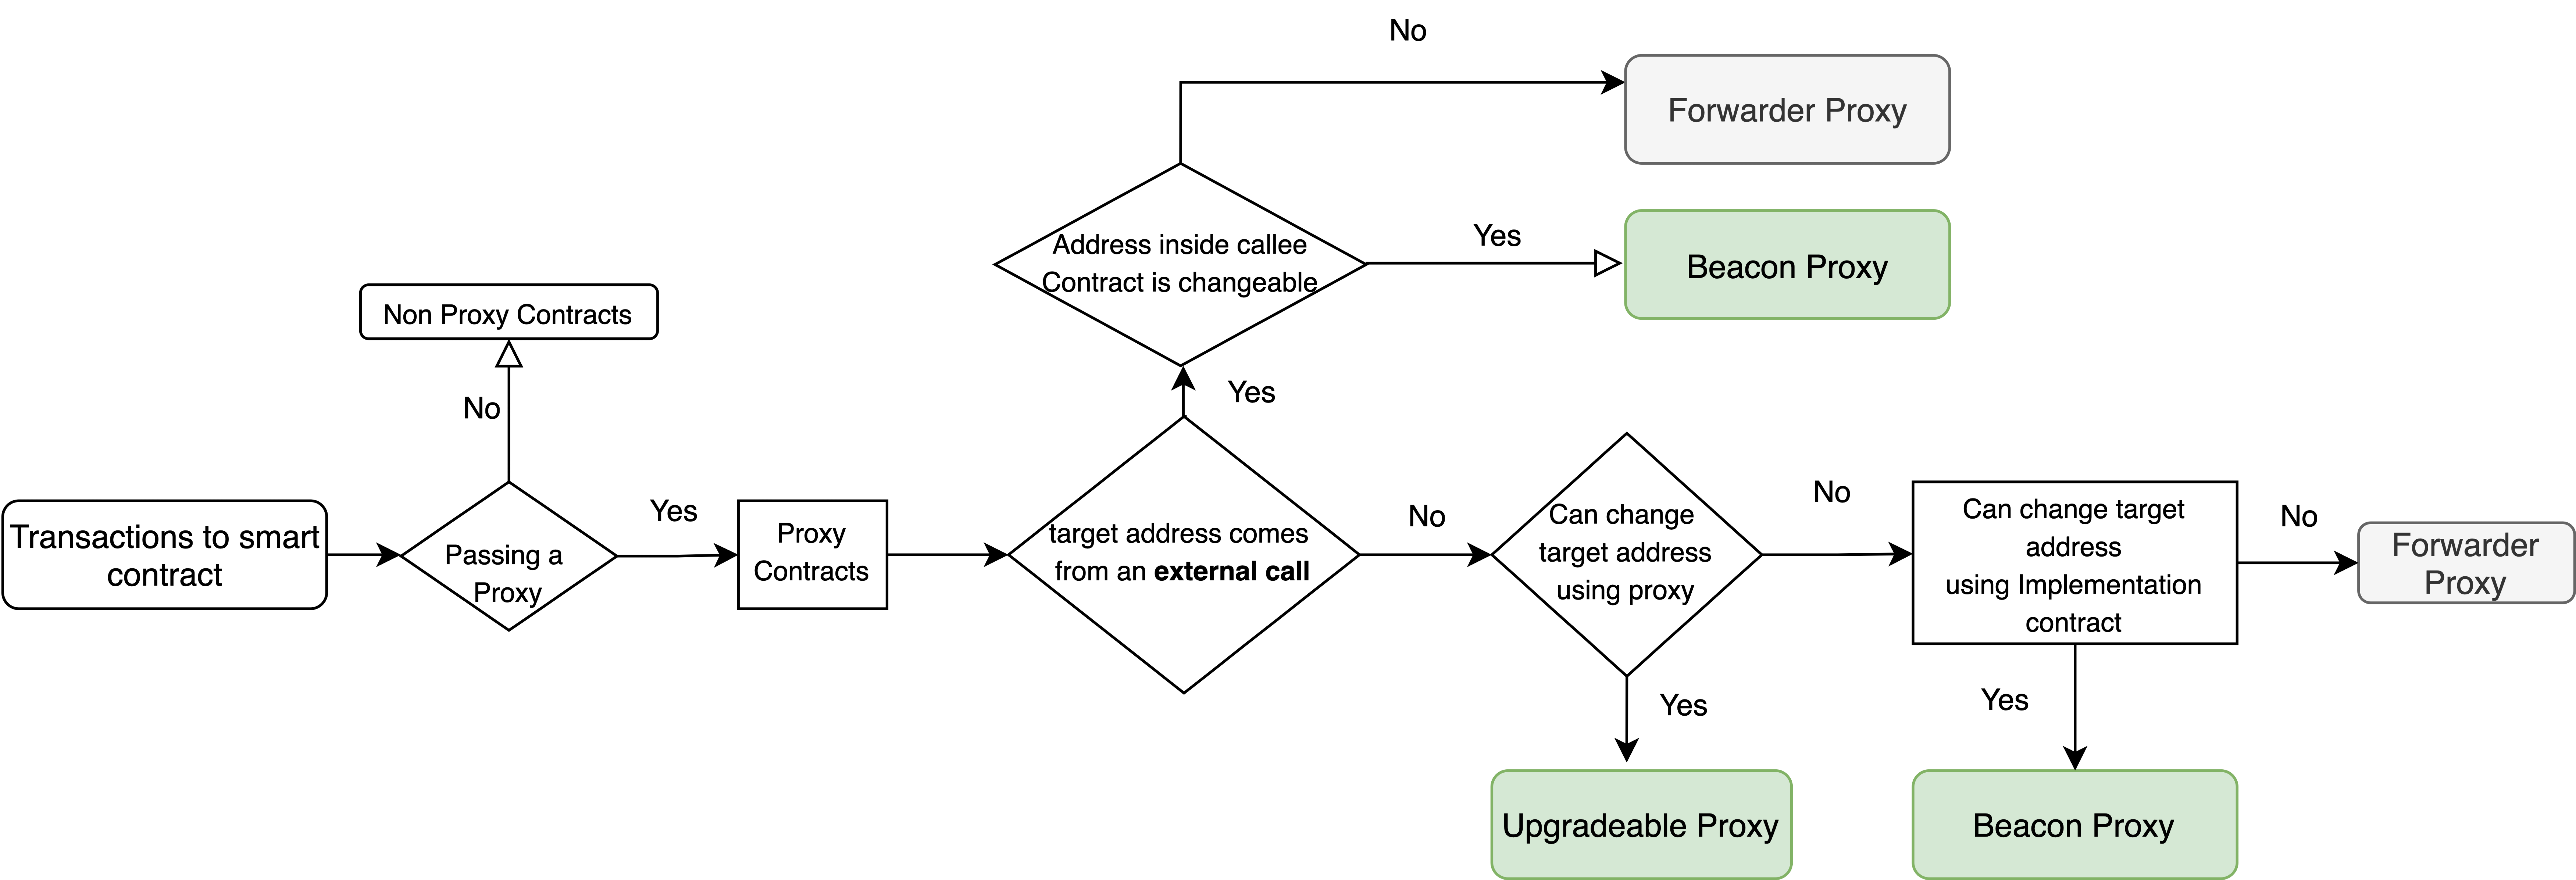
\includegraphics[width=1\textwidth]{New-method.png}\label{flowchart}
  \caption{Flowchart of the Process}
\end{figure}



\subsubsection{Results}

Having access to an Ethereum full archival node, we have collected transaction traces of transactions included in 2,064,595 blocks of Ethereum blockchain, starting from block number \textit{\#10800000} to \textit{\#12864595}. It covers transactions on the Ethereum blockchain from \textit{Sep-05-2020} to \textit{Jul-20-2021}. 

%Having transaction traces and the actions of each transaction, we have collected \textit{From} address (address of sender of the transaction), \textit{To} address (destination address of the transaction) and \textit{Transaction Hash} of actions which has \textit{delegateCall} as their \textit{Call Type} and their input is the same as their previous action. As mentioned in the previous part the From addresses are the address of the proxy contracts.

Applying our methodology gives us \textit{1,427,215} unique proxy contracts. However, a bunch of these proxies is using shared implementation contracts. We decide to weed out the proxy contracts that share the same implementation contract; however, two different Dapps may use the same implementation contract. The reason for this decision is that there are some Dapps like opensea~\footnote{\url{opensea.io}} that create proxy contracts for each of their user, and these proxies share the same implementation contract (it will reduce the redundancy). So after filtering proxies with the same implementation contracts, we come up with \textit{13,088} contracts.
Afterwards we filter \textit{Forwarder Contracts} from our dataset and then apply the first filter to check if the proxy contract has a method to change the target address. This filter finds \textit{7,470} regular upgradeable proxy contracts.
On the other hand, checking the remained proxy contracts (the proxies that neither forwarders nor regular upgradeable proxies) by applying the next filters explained in the methodology section, \textit{403} upgradeable proxy contracts found that follow Universal Upgradeable Proxy Pattern and also \textit{352} unique beacon proxy contracts.

At the end we find \textit{8,225} unique upgradeable proxy contracts with unique implementation contract. We randomly sampled 150 contracts from these contracts and manually checked them, and all of them were upgradeable proxy contracts. On the other hand, we sampled 150 contracts from those marked as non-upgradeable and checked them manually. Between these 150 contracts, just two were upgradeable. Our model did not catch these contracts because a failure happened on the decompiler to decompile the implementation contract code, so our assignment checker detector could not catch them. The reason is that implementation contracts are much larger in contrast with the proxy contract itself.


\section{Finding Admin of the Proxies}
\label{sec:governance}

This section proposes a novel way to find the admin of the proxy contract (the agent responsible for upgrading the proxy contract) and classify them based on their account type. We apply the method to the dataset of proxy contracts we provided from the previous section~\ref{sec:proxyFinding}. We also shed light on the risks regarding the number of decision-makers who have the authority to change the whole logic of the Dapps that are using a proxy contract.

The question we will answer in this part is who can upgrade the system? There should be an agent who decides on the upgrades of the system. Generally, there are three main types of admins for upgradeable smart contracts which we describe below; an Externally Owned Account (EOA), Multi-Signature wallets, and Governance schemes. EOA and multi-signature schemes add centralization risks to the system because a limited number of private keys can change the system's whole logic. Based on \textit{The State of DeFi Security 2021}~\cite{certikReport} report by Certik~\footnote{\url{certik.com}}, \textbf{Centralization} is the most common attack vector of the hacked DeFi projects. In further part of this section, we will explain a real-world incident to show how using an EOA as the admin of an upgradeable proxy contract may lead to loss of funds.

\textit{Externally owned Address(EOA):}
This most centralized way to deal with admin is to have just one private key controlling the upgrades. Using EOA as admin is the fastest way to respond to incidents, but in case of a malicious admin or a private key compromise, the whole funds are at risk.

\textit{Multi-Signature Wallet:}
A \textit{m out of n} Multi-signature wallet is a smart contract that can execute a transaction only if m number out of a specified n EOAs agree and sign the transaction.
Using multi-sig as admin is a better way to the upgrade's decision-making than using an EOA. However, it may not be decentralized. The problem here is that the Ethereum accounts are pseudo-anonymous, and the identity behind addresses is not recognizable. So, the malicious developer team can keep at least m signatures out of n in their hands, and in the desired time, they can upgrade a system to a malicious version and steal the funds.
Also, there are some types of governance voting which is known by \textit{Off-chain Governance Schemes} in which users who hold governance tokens can signal their votes on proposals in an off-chain tool like \textit{Discord} or \textit{Snapshot} and then another agent which is a part of multi-signature schemes can put the results on-chain and execute the actions if needed.
We consider the off-chain governance in the Multi-sig category because, in the end, these multi-signature wallet owners are the only on-chain agents responsible for changing the system, and there is no way to enforce the signers to reflect the off-chain agreement results to the smart contract.

\textit{On-Chain Governance Voting:}
The most decentralized way to decide on a system change is to use a decentralized voting scheme. This can be done by distributing governance voting tokens to the community, and then they can vote on a change proposal by staking their voting token. 
There is some critique to this method. Governance by voting has an inherent time delay to the upgrading process. This raises a problem when the system needs an instant upgrade (e.g., responding to an incident) \footnote{This arises the need for another mechanism to quickly fix bugs and upgrade the system in the event of incidents in conjunction with the voting process (e.g., Global shutdown in MakerDAO).}
It is also not cost-efficient for the voters because all token holders must send a transaction for voting and pay a network fee.
The other problem with this method is a fair distribution of the tokens. If the governance tokens are not distributed fairly, and the majority of tokens are granted to a limited number of users, they can change the voting results to their desired outcome.

\subsection{Exploring Admin Types}
As described above, proxy contracts may have three types of admin: EOA, Multi-Sig, and Governance Contract. In EOA and Multi-sig types, a person or a limited number of persons may decide to take control of the system. The risks regarding each admin type discussed above bring us to find the admin types of all proxy contracts we found in our first analysis.

In the previous section~\ref{sec:proxyFinding}, we gathered \textit{7,470} regular upgradeable proxy contracts. In this part, we try to find the admin of each proxy contract and recognize the type of the admin (i.e., EOA, Multi-Sig, Governance).
Here we describe our methodology of finding the admin addresses and their types. The process can be divided into two main parts: finding the admin account's address and finding the admin type (EOA, Multi-Sig, or decentralized governance).

\textbf{\emph{Finding the Admin Account's Address.}} EIP-1967~\cite{eip1967} suggested specific arbitrary slots for upgradeable proxy contracts to store \textit{Admin address}\footnote{Storage slot 0xb53127684a568b3173ae13b9f8a6016e243e63b6e8ee1178d6a717850b5d6103}. So, we first check this specific storage slot and if it is non-zero, the address that is saved inside it, is the admin address. 
However, not all proxy contracts use the EIP-1967 suggested storage slot. So, for non-EIP-1967 proxies, we propose a way to find the storage slot in which the admin address is stored. The process is very similar to how we found storage variable (slot) of the target address in~\ref{sec:proxyFinding}. We first find the function in which the admin can change the \textit{target address} (upgrade function). This function is critical and should only be called by the admin. It means there should be access control to check the caller of the function. We find this access control check, and conclude that the address that is checked inside, is the admin address.

\textbf{\emph{Finding the admin type.}} Having the admin address, we can check if the account is an EOA by just checking if the account consists of a code or not\footnote{using the \textit{eth\_getCode} method for the admin address}. If the contract does not contain code, the admin is an EOA and if it contains code, the admin is another smart contract which can be a multi-signature wallet. The most widely used multi-signature wallet is Gnosis Safe\footnote{\url{https://gnosis-safe.io/}} wallets. We automatically checked if the code of the admin address is the Gnosis multi-signature wallet, and if yes, we marked them as Multi-Signature admins. After picking Gnosis safe wallets, we manually checked 10\% of the remaining addresses to find any other patterns for multi-signature wallets and found other patterns (e.g., MultiSignatureWalletWithDailyLimit, etc.) and added them to the dataset as well. 

\textit{2,534} contracts between all \textit{7,470} proxies we have, are using another proxy contract as their admin, which is known as \textit{Admin Proxy}. Admin proxy contract adds another layer of indirection. In this case, the real admin (owner of the admin proxy) sends their desired transaction to the admin proxy, redirected to the primary proxy, and getting executed. So, we attempt to find the admin proxies among the admin addresses and then find the owner of these proxies. The owner's address is the real admin account that can upgrade these systems. Now that we have the admin address, we do the same processes as before to find the EOA and Multi-Signature types.
The remaining proxy contracts which are not marked as EOA or Multi-Signatures are marked as decentralized governance or unknown. We add unknown tag, because some of the contracts were using undefined new patterns as their multi-signature contracts and our model has false negatives to detect the multi-signatures. 
For a detailed explanation of the methodology and implementation, check the appendix.


By applying the above methodology in our dataset, the results show that out of \textbf{7,470} proxy contracts, \textbf{3,558} are controlled by an EOA address, \textbf{988} are controlled by a multi-signature wallet, and \textbf{2,924} addresses are either decentralized governance based admins, or unknown type.

The results show that a single EOA account controls 48\% of the proxy contracts and 61\% by an EOA or Multi-Signature wallets control. This is a significant risk to the Ethereum ecosystem because, in these contracts, one or a limited number of persons can decide to change the whole logic of the contract and take control of the funds under the custody of the contract.
Bent Finance incident~\cite{bentFinanceHack} is a real-world example of what may happen to all these proxy contracts. Bent Finance\footnote{\url{https://app.bentfinance.com/}} is a staking and farming platform. They are using \textit{Transparent Upgradeable Proxy} pattern in their system. The admin of the proxy was an EOA at the time of the incident. The malicious developer deployed a new implementation contract\footnote{\url{https://etherscan.io/address/0xb45d6c0897721bb6ffa9451c2c80f99b24b573b9}} in which it provides a huge amount of token to the malicious actor's address \footnote{0xd23cfffa066f81c7640e3f0dc8bb2958f7686d1f}. 
Afterward, the attacker upgraded the proxy to the malicious implementation contract, and by doing that, a considerable amount of tokens were assigned to the attacker's address. Once the balance was transferred to the attacker, they upgraded the proxy to the latest non-backdoor version to hide the exploit. 
Having a massive amount of tokens, the attacker drained liquidity from Curve Finance protocol, a decentralized exchange.
The same scenario may happen to all other upgradeable proxy contracts which use EOA or multi-signature wallets as their admin.


%We did not try to find the governance contracts because in the case of rug pulls only EOAs and Multi signature wallets are in a critical risk, so we did not attempt to recognize the governance contract admins. Also we should mention that our methodology failed in some cases due to the problems regarding the decompiler. In some cases the decompiler was not able to decompile the code or some part of the code which our code dropped those addresses as unknown results. 

%Implementation of Eternal storage in call based upgrades: https://medium.com/cardstack/upgradable-contracts-in-solidity-d5af87f0f913

\section{Concluding Remarks}

* Which update pattern is the best?
* Immutabilty is not a reality (cite Angela Welch?) 
* One approach is too find specifics of upgrade frameworks (libraries, implementations) that are commonly used, our approach is pattern-based and cross cuts different implementations. We demonstrated this to a leading blockchain firm in finding a broader set of contracts potentially volunerable to a bug in a commonly used UUPS libraries. 
* EOA -> the risk is underestimated -> stories -> that is a mess -> not centralized 
* Layer 2

%\subsection{Off chain upgrades (UNiswap Arbitrum)}: On-chain voting for an off-chain process. Other types of upgrade. Like front end changes etc.



%



\section{What is RB tokens}
%%"A currency, to be perfect, should be absolutely invariable in value," said David Ricardo in 1817.
%%There is a huge debate about the charectaristics of a stable asset. One may claim that a stable asset or currency is an asset that helps its owner to have stable purchasing power. Others may claim that an stable asset should have invariable quantity.

There is a growing tendency to issue asset on top of blockchain that represents  real world assets such as shares, commodities, and currencies. 

One way to implement this kind of tokens is that a company obtains a reserve of the asset and issue tokens that represents a unit of asset. But this design needs custodianship proofs, periodic audits and also trust on the third party.

The question raised here is whether it is possible to find a solution to remove the trust on the third party?

The answer is RB token Dapp. There are two parties involving on each contract of the system. The Red token holder who need a representation of the underlying asset on the blockchain, and Black token holder who bets against the pair value of ETH and the underlying asset.

Therefore, the amount of deposited ETH on each new agreement will grow or shrink depending on the exchange rates of the underlying asset and ETH. Because a blockchain has no inherent knowledge of exchange rates, this mechanism still requires one trustworthy entity called an oracle to write the exchange rates into the blockchain (or consensus can be taken across a set of oracles).

\emph{Working Example}: Assume Alice wants to create representation of Google share (GOOGL). She sets up a DApp that can hold ETH and issue tokens. The DApp determines how much ETH is equivalent to 1.5 GOGGL, using the current exchange rates, provided to the DApp by a trusted third-party oracle, and Alice deposits this amount of ETH into the DApp. The DApp issues to Alice two tokens, Red and Black. At some future time, the holder of Red token can redeem up to equivalent value of 1 GOOGL in ETH from the deposit and the holder of the Black token gets any remaining ETH. Alice will transfer the Black token to Bob who wants to bet against ETH/GOOGL. When Alice redeems the Red token, it will be worth 1 GOOGL in ETH when the entire deposit of ETH is worth more than 1 GOOGL. If the exchange rate of ETH drops enough or the exchange rate of the GOOGL raise enough (or combinatoion of them), the entire deposit will be worth less than a 1 GOOGL—Alice will get all of the deposit, and the holder of the Black token will get nothing.

There are two risks on the system: Volatility risk of ETH and the underlying asset. Decision on the system depends on the spot exchange rate of ETH and Underlying asset
($\frac{P_{ETH}}{P_{GOOGL}} $).


\section{Analysis}



\section{Systemization}
There are a number of stablecoins using crypto-assets as collateral to issue stablecoins which shows a very broad design landscape for indirectly-backed stable coins and different design goals and strategies behind stable coin systems. In this part we will discuss about the mechanism that could be added on top of the RBcoin system discussed on previous section that can be used to change the propetries of the system. The designer of a stable coin may have design goals like Fungibility(I think it should be removed)(Money like tokens could be replaced or sth like that), Stability, Simplicity, and Decentrality. 

Firstly, the designer sets the goals of the design and then assign the design parameters of the system to acheive the design goals.

In this part, we propose a systematical design-decision model for indirectly-backed stablecoins. The designer is facing four main design parameters to create a new indictly-backed stable coins which are Maturity date, Counter-party, Collateral risk and interventions. 



An overview of the indirectly-backed stablecoins design landscape is in Figure\ref{land}.

\begin{figure} 
\centering
\includegraphics[width=12cm]{Mindmap}
\caption{overview of the indirectly-backed stablecoins design landscape}
\label{land}
\end{figure}

\subsection{Maturity Date}
The indirectly backed stable systems are agreements between two different parties, a stable party and a volatile party. These two parties should be different because holding both sides of the contract is equal to keeping the underlying asset on the wallet and it is not logical to participate on such a system to just keep the asset.

In this agreement the parties agree to split their deposited asset at a specified date named maturity date. At the maturity date the stable party will receive an exact amount of underlying asset based on the price of the asset at the settlement date and the volitile party will receive the remained part.

The first parameter that the designer should decide about is the maturity date. The maturity could be happened at a fixed specific time or could be perpetual.
\subsubsection{Fixed Maturity dates}
The designer can set specific dates for the contracts to be matured for example at the first day of each months. At the day of maturity the deposited assets are devided into two parts. The \$1 equivalent amount of the asset goes to the pocket of the stable party (if possible) and the remained is for volatile party. This is simlar to futures contract in Finance.

The designer may let one of the parties to exercise the contract beforr the maturity date. It is very similar to american options. The exerciser could be the black coin holder, red coin holder or both of them. 

\subsubsection{Perpetual contracts}
The other way to design the stable coin contracts is to make them as a perpetuty. In this mechanism there is no specific day for the parties to mature the contract. The system may have the option of settlement.

The perpetual stable coin without settlement is not rational because it is like burning the underlying asset to issue stable coins. 

For open-ended perpetual stable coins one of the parties has right to request for settlement whenever she wants. The exerciser could be black coin holder or red coin holder.
\subsection{Counter party}
One of the design parameters is to decide who is the risk taker in each contract. Each newly issued contract is backed by a different vault. Each black coin points its vault because the amount of deposits depend on the black coin holder decision. 
The designer could decide whether use a pool for red coins or pair each red coin to its related black coin.

\subsubsection{Pooled}

In this type of design the black coins are pointing to the vaults. Red coins are fungible on the system and there is no differences between them. There is no relations between red coin and the black coin. 

In this class, all red coin holders are risk takers of the system and on the unexpected events the take the risks regardless of their issuance contract.

In this case a black coin holder do not know the counterparty and the risk is pooled here.

\subsubsection{Paired}

The designer can create a system in which each red coin and black coins are paired and point to the issued contract. Now the black coin holders now their counterparty and the red coin holder is the risk taker of its own vault. So the risk is not pooled here.
\subsection{Collateral Risk}
If the price of the underlying asset goes down, the value of deposit falls below collateral ratio. The designers have the choice to react to this situation. We described some of different possible decisions:

\paragraph{Liquidation}
This variety of design is similar to the marginal accounts in traditional finance. If the underlying asset decreases in price and the value of a vault runs under the collateralization ratio, the system will liquidate the vault.

Liquidation occurs in the case that a vault is the danger area and may not able to pay its obligation. The deposited assets will transfer to the person who takes the responsibility of the debt of the vault. In other words, the liquidator should pay the borrowed red coin (and other obligations in a type of design, such as stability fee in MakerDAO) and receive the vault in exchange.


In liquidation design, the majority of vaults are over-collateralized. If a vault goes under-collateralize it will be liquidated. So, the red coin holders are pretty sure that their coin is backed by a dollar (. They can exchange their asset because the red coins are similar.

Smart contracts cannot trigger themselves. So, there should be an outsider player (like Keepers in MakerDao) to liquidate the warned vaults. They should trace the system to find the under-collateralized vaults and call the liquidation function. Then the keeper will transfer the debt of the vault to the smart contract and receive the deposit of the vault in exchange.

There are design parameters in the liquidation method:

\begin{enumerate}
  \item Collateralization Ratio:
This number shows the factor of over-collateralization. The ratio between the value of the deposits on each vault and the value of borrowed red coins should always be more than the collateralization ratio.
  
The collateralization ratio is depending on the volatility of the underlying asset. For instance, in the MakerDAO platform, the collateralization ratio for ETH vaults is 1.5. However, in the Synthetix project, it is 7.5 for SNX token, which is more volatile than ETH.
  \item Liquidation Incentive:
A smart contract is not able to trigger itself. An outsider player named liquidator should pay the transaction fee to call the liquidation function of the smart contract. Some factors influence the costs and profit of liquidators:
\begin{enumerate}
	\item Transaction fee:
The liquidator should trigger the liquidation function, send the sufficient red coins, and bid on the auction to win the vault. The user has to pay the transaction fee for these processes. The transaction fee depends on the time of transaction and network congestion.  
	\item Cost of capital: The liquidator pays the obligation by Red coin and receives the deposited coins of the vault. Therefore, the liquidator needs a sufficient amount of red coins for liquidation. There is an opportunity cost associated with the decision of the liquidator to not lend her capital and gain interest.

In other scenarios, the liquidator may just borrow the fund from lending platforms to liquidate the vault and pay back the loan afterward. There is a cost of borrowing in this scenario as well. So, there is a cost of capital for the liquidator.
	\item Price Oracles: RB coin systems need the price of the underlying asset in USD. Blockchains have no access to externals data. Oracles are outsider systems that collect the price and push them to the blockchains. Price inefficiency may impose extra costs on the liquidator. For instance, if the price of the asset is \$100 on the markets, although the oracle price is \$90, the liquidator spends more to provide liquidity from the markets.
\end{enumerate}  

The designer has to incentivize the liquidators to trace the blockchain, find alerted positions, and then send transactions to liquidate them. 

The mechanism of the incentivization is varied between protocols. A majority of platforms give the liquidator discounts on the vaults. For instance, in Single Collateral DAI (SAI), there was a \%3 discount on the liquidation process. Other platforms are using auction models to let the market decide about the value of the vault. 
  
  \item Auction model:
In the case of liquidations,  liquidators may come up with a specific warned position and want to liquidate it. The system designer has different options for the decision of picking the winner liquidator.
 
The simplest implementation mechanism is the First Come First Serve. However, it won't be fair for the vault holder if the first liquidator bids with a low amount of red coins.

There are other auction-based mechanisms to find the liquidator. The question raised here is, which method is the most efficient and fair auction model for both bidders and vault holders.

MakerDao utilizes a mixture of an absolute-auction and a reverse-auction model for the liquidation process.

The absolute auction model is used until the bids cover the debt of the vault. When the bids pass the debt, the auction reversed, the bidders bid on a lower amount of the deposits on the vault for a specific amount of DAI tokens, specified on the absolute auction step.
  
  \item Liquidation penalty:
The liquidation penalty is an extra punishment for the black coin holders to care about their debt to collateral ratio.
MakerDAO platform charges liquidated vault extra \%13 as a punishment for their vault holders. There are two main reasons to add Liquidation penalty on the design:

\begin{enumerate}

  \item To force vault keepers to be over-collateralized
  \item To mitigate grinding attacks: grinding attack occurs when the position holder deliberately unsafe her black coin and participate in the liquidation auction against her position to buy her deposited assets cheaper.

\end{enumerate}
\end{enumerate}

Using liquidation mechanism as a shield to protect the system provoke criticism. Possibly the black coin holders are freaking out when the price of ETH drops significantly. They may proceed to net out just before the liquidation occurs to their vaults. We called this situation "early liquidation" of the system. 

In this case, the system needs more ETHs to be deposited. The liquidation mechanism is designed to force the black coin holders to inject more ETHs to the system, but the black coin holders withdraw their deposits, and the total collateral of the system drops significantly, which is not the goal of the designers in this situation.

\paragraph{Withholding rewards}

Majority types of designs like liquidation are disincentivizing bad actors. But, another approach is to encourage users to act properly and incentivizing good actors of the system.

For instance, in the Synthetix project users need collateralize SNX tokens (Synthetix network token) to receive sUSD tokens (Synthetix stable coin pegging a USD). There is no margin call methods or liquidation function on the design. But, there is a reward on the system for users who keep more than the over-collateralization ratio. 
The Synthetix system has \%2 annual inflation on SNX tokens. The inflationary tokens are allocated to the vaults that hold more than the collateralization ratio.

There is another reward for the system. The traders on the exchange of the Synthetix project, pay transfer fees collected and distributed to the vaults holding more than the collateral ratio.

The system incentivizes people to stake their SNX token to be over-collateralized and receive the rewards. So, there is no punishment in the system for bad actors in this class of design.

\paragraph{Banning Black coin holders}

In the design of indirectly-backed stable coins, the red coins are not redeemable. In other words, the red coin holders cannot give back their red coins to receive \$1 of the deposited ETH in exchange. The red coin holder must own (or buy if possible) a black coin to net out a vault and receive the ETH.

In the liquidation scenario, the designer pushes black coin holders to be over-collateralized, applying liquidation punishments. Red coin holders and arbitragers are confident that there is no difference between the red coins because each of the red coins is backed by a sufficient amount of ETHs to be \$1 (with high probability).

In another class, the designer removes the liquidation mechanism, prevent black coin holders from withdrawal. In the fungible black coin design class, the designer also forbids the black coin holders from transferring their token. 

In this situation, the incentives for black coin holders to be over-collateralized has been decreased, compared to liquidation design class. But, there is a huge incentive left for them to be over-collateralized. If the price of the underlying asset drops, the black coin holders may want to sell their deposited assets to reduce the loss. In this scenario, just black coin holders that have over-collateralized vaults can net out and receive their underlying assets to sell them to the market.

This type of design will increase the fluctuation of the price of the red coin. The market watches the aggregated collaterals on the system and the number of red coins issued by the system and also the price of the underlying asset to evaluate the price of red coins. So when the price of underlying asset drops, the price of red coins will reduce concerning the underlying asset price. 

In this scenario, red coin holders are taking parts of the risk of underlying asset volatility risk. On the situation that the price of the asset drops significantly, the value of the stable coin will fall.

\paragraph{Reputation systems}

In traditional finance, reputation scoring systems are used to decrease or eliminate the collateral needs for a specific financial transaction. Participants are utilizing their reputation as collateral or source of trust for financial services. 

For instance, in the FICO credit score system, users can enhance their credit limit by increasing their credit score. There is a default risk on credit systems, but the defaulted person will be punished by credit score reduction. The bad actor loses reputation scores forbidden from using plenty of financial services. Therefore, users have adequate incentives to pay their bills.

A revolution of decentralizing the finance products on top of blockchain technologies began in early 2018, named Decentralized Finance (Defi) movement. There is a myriad of different decentralized financial services out there, such as MakerDAO, Compound, Synthetix, Aave, etc. 

There are no differences between users that act properly on Defi platforms and the bad actors. The DeFi ecosystem suffers from a lack of a reputation system or reputation scoring. Using a reputation system will incentivize users to act properly and also reduce the default risk of the system. On the other side of the coin, the users with high-grade reputation scores have new opportunities. So, the cost of defaulting will be increased for high-grade users.

There are barriers to implementing an effective reputation system on blockchains. Lack of strong identities or anonymity is one of them. Also, users can create fake histories. However, these are not impossible to address.

In case that our system concludes a trustworthy reputation system, the designer can use reputation as collateral.  We describe two different designs using reputation systems:
\begin{enumerate}
	\item Reputation-based collateral ratio: 
In the design of the system, the collateral ratio could be reliant on the reputation of the user. In other words, the collateral ratio is higher for new users (users with no reputation) and lower for users that act properly for a long time.
	\item Reputation-based staibility fee
In systems like MakerDAO, the DAI borrowers are obliged to pay a fee on their borrowing named stability fee. This stability fee is being set by Maker token holders.
	In a design based on the reputation, the stability fee could be dependent on the reputation of the user. The reputable user is paying a lower stability fee compared to the new users.
\end{enumerate}
 
\paragraph{Insurance}
Insurance models are used to hedge the risk of unexpected events in different systems. Under-collateralization of a vault is an unexpected event on the RBcoin system. The designer could use an insurance model to protect parties from financial loss in the case of under-collateralization. 

On the insurance model, the insurer will pay a premium to the insurance company. The company will protect the client from financial loss. 

In RBcoins there could be a built-in or outsourced insurance model to protect parties from under collateralization loss. The question raised here is who should pay the premium.

\begin{enumerate}
	\item Premium pay by Red coin holders:
It is very similar to Credit Default Swaps (CDS) on traditional finance. In this design, the approach is that the red coin holders are lending some amount of money to black coin holders. Therefore, black coin holders are borrowing from red coin holders to have a leveraged position on the underlying asset. In this situation, the red coin holders can pay an insurance premium to the contract to protect themselves from the default risk of black coin holders. In the case of under-collateralization, if the black coin holder cannot afford the loss, the insurance contract will pay the loss to the red coin holder.

This type of design is implemented on the MakerDAO platform. The DAI borrowers are paying a premium so-called stability fee to the system. These fees are collected on a pool named Maker Buffer pool. In the case of liquidation of a CDP, if the winner of the auction pays a lower amount of the obligation of the vault, the difference between the obligation and the paid amount will be paid by the Maker Buffer pool.

	\item Premium pay by Black coin holders
In this type of design, the black coin holders are paying the insurance premium. It is similar to regular insurance contracts in which the insurer buys an asset and guarantee it by paying a premium to insurance companies. For example, a person purchases a house and insure it.
Here the black coin holders are buying a position and pay the insurance premium. If the price of underlying asset drops and the vault going to be liquidated the insurance contract will pay on behalf of the insurer.
	\item Premium pay by both
In this scenario, both Red and Black coin holders are paying the insurance premium to ensure their positions. 
\end{enumerate}
\subsection{Intervention}

The designer should indicate the level of intervention on the system. There could be some mechanisms to change the level of properties on the system. For instance, the designer may use interest rate models, algorithmic models or secondary tokens to acheive a system property.

\subsubsection{Float}

The desiner may let the system to be free of human or algorithm intervenions. This is the most decentral type of design. This type of design benefits simlicity and decentrality but the red coins has fluctuations.

\subsubsection{Interest rate models}

Interest rates are tools that a system governer has to stimulate the demand or supply side of a system. The designer of indirectly-backed stable coins can use interest rate models on red coins or black coins (two different rates) to adjust the supply and demand of black coins and red coins in the system. This rates could be adjusted by human intervention like DAI or could be fully algorithmic.

\subsubsection{Parameter setting}

All types of the indirectly-backed stable coin system has some parameters in common such as collateral ratio. In specific designs, there are other design parameters added to the system such as maturity dates, insurance premium and rates. The designer may decide to intervene on the system and change these parameter over time. This intervention could be by humans or algorithmic. 

\subsubsection{Issue haircut}

The designer should indicate that in case that the price of underlying asset goes down, who is the risk taker of the system. On regular system risk taker of the system is black coin holders till the price falls strongly and the black coins worth zero, then the red coin holders take all the risk.

The designer has other option to divide the risk between red coin holders and black coin holders. The designer could set hair cut parameter a (< 1). It means that if the price of the underlying asset falls 1 percent the redcoin holder now takes a percent of the risk and the the black coin holder takes 1-a percent.

This haircut parameter could be changed during the time by human intervention or algorithmic.


\subsubsection{Algorithmic rebasing models}

The designer may use rebasing models to change the number of tokens in a way that at the end of each day the price of redcoins is exactly a dollar.

%\section{Design Landscape}
The purpose of designing a crypto-asset backed stablecoin is to create a stable asset out of a volatile asset. There are a number of stablecoins using crypto-assets as collateral to issue stablecoins which shows a very broad design landscape for indirectly-backed stable coins.

In this part, we propose a systematical design-decision model for indirectly-backed stablecoins. There are some key design decisions for each core feature. We describe core features and the key design decisions related to the main features, and also we will discuss the pros and cons of each feature.

An overview of the indirectly-backed stablecoins design landscape is in Figure \ref{land}.

\begin{figure*} [ht]
\centering
\includegraphics[width=16cm]{Mindmap}
\caption{overview of the indirectly-backed stablecoins design landscape}
\label{land}
\end{figure*}

\section{Fungibility}
Fungibility or Interchangeability refers to the feature of an asset to be exchanged by the same asset type with equal quality and quantity. For instance, dollar bills are fungible because people can exchange the same amount of dollars without any frictions.

The first design decision is whether the tokens on the systems should be fungible or should be non-fungible. 

Fungiblity decision is devided into two parts:
\begin{itemize}
  \item Red coins Fungibility
  \item Black coins Fungibility
\end{itemize} 
We will discuss them seperately on next sections.


\subsection{Red coins Fungibility}
The Red coins, the stable coin of the system, could be fungible or non-fungible. All currently implemented indirectly-backed stablecoins are using fungible stablecoin design. However, it could be non-fungible as well.

\subsubsection{Non-fungible Red coins}
A stablecoin system designer could allow red coins to be non-fungible. For instance, each token could be backed by a different amount of ETHs without limitations on the system such as collateral ratio, liquidation and etc.

In this design class, the Red coin and Black coin should be pair-wise. Because each pair is backing by a different vault and a specific amount of deposited ETH.

There should be a system parameter for each red coin, depends on its vault to distinct the coins.
For example, each red coin could be marked by debt to collateral ratio, the number of minted red coins divided by the value of deposited ETH on the related vault, which clarifies the safeties of the coin.
So the buyer could have speculation on the price of each red coin base on the debt to collateral ratio.

Some reasons push designers to make red coins fungible. The first reason is usability. Assume that Alice wants to buy 100 red coins. On the other side, Bob wants to sell just 30 coins, Carol wants to sell 50 and David wants to sell 20 red coins. Now Alice should make a price speculation of three different coins and buy them at different prices which is not convenient for her.

The other issue with the non-fungible red coins is price discovery. Markets and crowd wisdom help to aggregate different opinions on the value of an asset. The aggregated results will discover the efficient price of the asset. In non-fungible design, there is not a straight relation between the price of each red coin and the specific characteristic of them like the debt to collateral ratio. So, Each person has speculation for each coin. Because of non-fungibility, the aggregations would not happen and so the real price will not be discovered.

The other reason is that stable coin users are willing to use the stable coins as a money. So, they need stable coins serve as a unit of account which means that you can price other goods or assets using the stable coin. In non-fungible design each red coin has a specific price. So, users can not price other goods based on the stable coin.


\subsection{Fungible Red coins}
As mentioned in the previous part, stable coin designers put all their effort to create stable coin systems including fungible red coins. There are different mechanisms to bring fungibility into red coins. We classify them into two key designs discussed in the next sections.

\begin{itemize}
  \item Under-collaterallization
  \item Separate maturity dates
\end{itemize} 


\subsubsection{Collateral Value Assurance}

One of the methods to bring fungibility into red coins is to set a lower limit for vaults (Collateralization ratio). If the value of deposited ETH in a vault drops beneath a specific amount, then the system decides to take an action. 

In this circumstance, there is a minimum amount of ETHs (collateral ratio)  backing each red coin. It secures the fungibility of red coins. Red coin holders are sure that there is at least a dollar in the vault for their red coin  (strongly expected). There is no difference between their red coin and the red coin of other people in this circumstance.

We will discuss various designs that differ on how they secure the vaults from the under-collateralization in the next sections. Some of them are incentivizing vault keepers to keep their deposit more than collateralization ratio and some of them are disincentivizing the bad actors of the system.
 
\paragraph{Liquidation}
This variety of design is similar to the marginal accounts in traditional finance. If the underlying asset decreases in price and the value of a vault runs under the collateralization ratio, the system will liquidate the vault.

Liquidation occurs in the case that a vault is the danger area and may not able to pay its obligation. The deposited assets will transfer to the person who takes the responsibility of the debt of the vault. In other words, the liquidator should pay the borrowed red coin (and other obligations in a type of design, such as stability fee in MakerDAO) and receive the vault in exchange.


In liquidation design, the majority of vaults are over-collateralized. If a vault goes under-collateralize it will be liquidated. So, the red coin holders are pretty sure that their coin is backed by a dollar (. They can exchange their asset because the red coins are similar.

Smart contracts cannot trigger themselves. So, there should be an outsider player (like Keepers in MakerDao) to liquidate the warned vaults. They should trace the system to find the under-collateralized vaults and call the liquidation function. Then the keeper will transfer the debt of the vault to the smart contract and receive the deposit of the vault in exchange.

There are design parameters in the liquidation method:

\begin{enumerate}
  \item Collateralization Ratio:
This number shows the factor of over-collateralization. The ratio between the value of the deposits on each vault and the value of borrowed red coins should always be more than the collateralization ratio.
  
The collateralization ratio is depending on the volatility of the underlying asset. For instance, in the MakerDAO platform, the collateralization ratio for ETH vaults is 1.5. However, in the Synthetix project, it is 7.5 for SNX token, which is more volatile than ETH.
  \item Liquidation Incentive:
A smart contract is not able to trigger itself. An outsider player named liquidator should pay the transaction fee to call the liquidation function of the smart contract. Some factors influence the costs and profit of liquidators:
\begin{enumerate}
	\item Transaction fee:
The liquidator should trigger the liquidation function, send the sufficient red coins, and bid on the auction to win the vault. The user has to pay the transaction fee for these processes. The transaction fee depends on the time of transaction and network congestion.  
	\item Cost of capital: The liquidator pays the obligation by Red coin and receives the deposited coins of the vault. Therefore, the liquidator needs a sufficient amount of red coins for liquidation. There is an opportunity cost associated with the decision of the liquidator to not lend her capital and gain interest.

In other scenarios, the liquidator may just borrow the fund from lending platforms to liquidate the vault and pay back the loan afterward. There is a cost of borrowing in this scenario as well. So, there is a cost of capital for the liquidator.
	\item Price Oracles: RB coin systems need the price of the underlying asset in USD. Blockchains have no access to externals data. Oracles are outsider systems that collect the price and push them to the blockchains. Price inefficiency may impose extra costs on the liquidator. For instance, if the price of the asset is \$100 on the markets, although the oracle price is \$90, the liquidator spends more to provide liquidity from the markets.
\end{enumerate}  

The designer has to incentivize the liquidators to trace the blockchain, find alerted positions, and then send transactions to liquidate them. 

The mechanism of the incentivization is varied between protocols. A majority of platforms give the liquidator discounts on the vaults. For instance, in Single Collateral DAI (SAI), there was a \%3 discount on the liquidation process. Other platforms are using auction models to let the market decide about the value of the vault. 
  
  \item Auction model:
In the case of liquidations,  liquidators may come up with a specific warned position and want to liquidate it. The system designer has different options for the decision of picking the winner liquidator.
 
The simplest implementation mechanism is the First Come First Serve. However, it won't be fair for the vault holder if the first liquidator bids with a low amount of red coins.

There are other auction-based mechanisms to find the liquidator. The question raised here is, which method is the most efficient and fair auction model for both bidders and vault holders.

MakerDao utilizes a mixture of an absolute-auction and a reverse-auction model for the liquidation process.

The absolute auction model is used until the bids cover the debt of the vault. When the bids pass the debt, the auction reversed, the bidders bid on a lower amount of the deposits on the vault for a specific amount of DAI tokens, specified on the absolute auction step.
  
  \item Liquidation penalty:
The liquidation penalty is an extra punishment for the black coin holders to care about their debt to collateral ratio.
MakerDAO platform charges liquidated vault extra \%13 as a punishment for their vault holders. There are two main reasons to add Liquidation penalty on the design:

\begin{enumerate}

  \item To force vault keepers to be over-collateralized
  \item To mitigate grinding attacks: grinding attack occurs when the position holder deliberately unsafe her black coin and participate in the liquidation auction against her position to buy her deposited assets cheaper.

\end{enumerate}
\end{enumerate}

Using liquidation mechanism as a shield to protect the system provoke criticism. Possibly the black coin holders are freaking out when the price of ETH drops significantly. They may proceed to net out just before the liquidation occurs to their vaults. We called this situation "early liquidation" of the system. 

In this case, the system needs more ETHs to be deposited. The liquidation mechanism is designed to force the black coin holders to inject more ETHs to the system, but the black coin holders withdraw their deposits, and the total collateral of the system drops significantly, which is not the goal of the designers in this situation.

\paragraph{Withholding rewards}

Majority types of designs like liquidation are disincentivizing bad actors. But, another approach is to encourage users to act properly and incentivizing good actors of the system.

For instance, in the Synthetix project users need collateralize SNX tokens (Synthetix network token) to receive sUSD tokens (Synthetix stable coin pegging a USD). There is no margin call methods or liquidation function on the design. But, there is a reward on the system for users who keep more than the over-collateralization ratio. 
The Synthetix system has \%2 annual inflation on SNX tokens. The inflationary tokens are allocated to the vaults that hold more than the collateralization ratio.

There is another reward for the system. The traders on the exchange of the Synthetix project, pay transfer fees collected and distributed to the vaults holding more than the collateral ratio.

The system incentivizes people to stake their SNX token to be over-collateralized and receive the rewards. So, there is no punishment in the system for bad actors in this class of design.

\paragraph{Banning Black coin holders}

In the design of indirectly-backed stable coins, the red coins are not redeemable. In other words, the red coin holders cannot give back their red coins to receive \$1 of the deposited ETH in exchange. The red coin holder must own (or buy if possible) a black coin to net out a vault and receive the ETH.

In the liquidation scenario, the designer pushes black coin holders to be over-collateralized, applying liquidation punishments. Red coin holders and arbitragers are confident that there is no difference between the red coins because each of the red coins is backed by a sufficient amount of ETHs to be \$1 (with high probability).

In another class, the designer removes the liquidation mechanism, prevent black coin holders from withdrawal. In the fungible black coin design class, the designer also forbids the black coin holders from transferring their token. 

In this situation, the incentives for black coin holders to be over-collateralized has been decreased, compared to liquidation design class. But, there is a huge incentive left for them to be over-collateralized. If the price of the underlying asset drops, the black coin holders may want to sell their deposited assets to reduce the loss. In this scenario, just black coin holders that have over-collateralized vaults can net out and receive their underlying assets to sell them to the market.

This type of design will increase the fluctuation of the price of the red coin. The market watches the aggregated collaterals on the system and the number of red coins issued by the system and also the price of the underlying asset to evaluate the price of red coins. So when the price of underlying asset drops, the price of red coins will reduce concerning the underlying asset price. 

In this scenario, red coin holders are taking parts of the risk of underlying asset volatility risk. On the situation that the price of the asset drops significantly, the value of the stable coin will fall.

\paragraph{Reputation systems}

In traditional finance, reputation scoring systems are used to decrease or eliminate the collateral needs for a specific financial transaction. Participants are utilizing their reputation as collateral or source of trust for financial services. 

For instance, in the FICO credit score system, users can enhance their credit limit by increasing their credit score. There is a default risk on credit systems, but the defaulted person will be punished by credit score reduction. The bad actor loses reputation scores forbidden from using plenty of financial services. Therefore, users have adequate incentives to pay their bills.

A revolution of decentralizing the finance products on top of blockchain technologies began in early 2018, named Decentralized Finance (Defi) movement. There is a myriad of different decentralized financial services out there, such as MakerDAO, Compound, Synthetix, Aave, etc. 

There are no differences between users that act properly on Defi platforms and the bad actors. The DeFi ecosystem suffers from a lack of a reputation system or reputation scoring. Using a reputation system will incentivize users to act properly and also reduce the default risk of the system. On the other side of the coin, the users with high-grade reputation scores have new opportunities. So, the cost of defaulting will be increased for high-grade users.

There are barriers to implementing an effective reputation system on blockchains. Lack of strong identities or anonymity is one of them. Also, users can create fake histories. However, these are not impossible to address.

In case that our system concludes a trustworthy reputation system, the designer can use reputation as collateral.  We describe two different designs using reputation systems:
\begin{enumerate}
	\item Reputation-based collateral ratio: 
In the design of the system, the collateral ratio could be reliant on the reputation of the user. In other words, the collateral ratio is higher for new users (users with no reputation) and lower for users that act properly for a long time.
	\item Reputation-based staibility fee
In systems like MakerDAO, the DAI borrowers are obliged to pay a fee on their borrowing named stability fee. This stability fee is being set by Maker token holders.
	In a design based on the reputation, the stability fee could be dependent on the reputation of the user. The reputable user is paying a lower stability fee compared to the new users.
\end{enumerate}
 
\paragraph{Insurance}
Insurance models are used to hedge the risk of unexpected events in different systems. Under-collateralization of a vault is an unexpected event on the RBcoin system. The designer could use an insurance model to protect parties from financial loss in the case of under-collateralization. 

On the insurance model, the insurer will pay a premium to the insurance company. The company will protect the client from financial loss. 

In RBcoins there could be a built-in or outsourced insurance model to protect parties from under collateralization loss. The question raised here is who should pay the premium.

\begin{enumerate}
	\item Premium pay by Red coin holders:
It is very similar to Credit Default Swaps (CDS) on traditional finance. In this design, the approach is that the red coin holders are lending some amount of money to black coin holders. Therefore, black coin holders are borrowing from red coin holders to have a leveraged position on the underlying asset. In this situation, the red coin holders can pay an insurance premium to the contract to protect themselves from the default risk of black coin holders. In the case of under-collateralization, if the black coin holder cannot afford the loss, the insurance contract will pay the loss to the red coin holder.

This type of design is implemented on the MakerDAO platform. The DAI borrowers are paying a premium so-called stability fee to the system. These fees are collected on a pool named Maker Buffer pool. In the case of liquidation of a CDP, if the winner of the auction pays a lower amount of the obligation of the vault, the difference between the obligation and the paid amount will be paid by the Maker Buffer pool.

	\item Premium pay by Black coin holders
In this type of design, the black coin holders are paying the insurance premium. It is similar to regular insurance contracts in which the insurer buys an asset and guarantee it by paying a premium to insurance companies. For example, a person purchases a house and insure it.
Here the black coin holders are buying a position and pay the insurance premium. If the price of underlying asset drops and the vault going to be liquidated the insurance contract will pay on behalf of the insurer.
	\item Premium pay by both
In this scenario, both Red and Black coin holders are paying the insurance premium to ensure their positions. 
\end{enumerate}

\subsubsection{Separate Maturity Dates}
This kind of design employs the idea of Futures in traditional finance. Each contract is an agreement between a volatile and a stable party. They deposit an amount of ETHs on the system (Q). The strike price (K) is the dollar value of ETHs that the parties agree that the stable player will receive at the maturity date (M). The remained ETHs on the vault will go to the pocket of the volatile party.

For a specific amount of pooled ETHs, two tranches are created, the stable token and a volatile token (black token). Tranching in traditional finance is used when several securities are created from a pool of other assets, carrying different risks. The junior tranche (volatile token) takes the majority of the risk and the senior tranche (stable coin) takes a lesser risk.  

The stable tokens are not fungible because each represents a different maturity date.  To create a fungible stable coin, the stable tokens with different maturities are bundled to create the Red coin, stable coin of the system. The amount of red coins each user receives is depending on the maturity date and the strike price of the deposited stable coin.

For example, in the Lien project, the agreement between parties is that at the maturity day, the stable token holder will receive k USD if the deposited ETH worth k USD, and the surplus will belong to the volatile token holder. If the value of deposited ETH dropped below k USD then the stable token worth below K USD and the volatile token worth zero. There are different specified maturity dates every 2 weeks. When a party receives a stable token, she will deposit it on a smart contract named iDOL to receive the stable coin (iDOL token). The iDOL contract bundles stable tokens with different maturities and strike prices and issues a stable coin out of this basket.


\subsection{Black coins Fungibility}

The Black coins, volatile coin of the system, could be fungible or non-fungible. 

\subsubsection{Non-fungible Black coin}

In the majority of implemented indirectly-backed stable coin systems, such as DAI and sUSD black coins are non-fungible. The vaults in these projects are covering various amounts of ETHs. Consequently, the vaults are not fungible. 

Non-fungibility of black coins is one of the primary obstacles of the currently implemented projects. These systems are designed to attract users who need stability along with the features of cryptocurrencies. 

If Alice decides to issue new stable coins, first she requires to create a pair of a red coin and a black coin. She obliged to keep the black coin because black coins are not transferable. So, the users that need stability should wait till another person who is willing to open a leveraged position, create a new vault, and want to sell her red coins to the market.

The other problem of this kind of design is the control of the demand and supply of stable red coins. If the demand for red coins suddenly increases in markets, the price of red coins in markets will be increased. This is an opportunity for arbitragers to make a profit because the price of red coins is pegging a dollar. The arbitragers issue new red coins that cost \$1, sell the red coins to the market to make a profit. But, the problem raised here, because if the arbitrager creates a new vault, then she should hold a non-fungible black coin position. So, the arbitragers are not confident about the price of the red coins. Therefore, there is no motivation for them to make arbitrage on red coin markets.
 
The designers of the MakerDAO platform are using interest rate models to control the supply and demand for red coins and black coins. This core design feature will be explained in detail, in the next sections.

\subsubsection{Fungible Black coin}

Making black coins fungible is the way to solve the mentioned problem. If Alice wants a red coin, she can open a new vault, sell her black coin to the market, and then decide to use it or keep her red coin.

The fungibility of black coins could boost the market capitalization of indirectly-backed stable coins because people who are willing to use stable coins can issue new stable coins without friction.

In this sort of design, there is no need to adjust interest rates to control the demand and supply of red coins because if the price of recoins increases in a market, the arbitragers can create new vaults, sell the issued black coin to the markets and sell the newly generated red coin, which worths a dollar, to a person who is buying them more than a dollar. The arbitrager also could implement these steps in just one transaction, using the meta transaction method to save money on the transaction fees.

The problem with this type of design is when the demand for red coins increases, and there is no demand for black coins. So, the arbitrager should sell the newly generated black coin lower than the issued price.

However, it uses free-market decisions to calculate the price of red and black coins, which means if the price of red coin increases and there is no demand for black coins, the price of red coins will exceed a dollar. 

The other problem with this type of design is the transaction fee for arbitragers. Because the arbitragers are using meta transactions, they should pay high transaction fees for the arbitrage, which may not be profitable in such cases.
\subsection{Underlying asset}
The first decision that a designer should take is choosing the asset that the issuer use as collateral to issue new stable coins.

There is a strong dependency between the risk related to the underlying asset and the design parameters of an indirectly-backed stable coin.

The stable coins could be backed by a single asset, like SAI (the first version of DAI), sUSD, USDx. Or by a basket of different crypto assets like DAI. In multi-collateral backed stable coins, several design parameters depend on the assets used as collateral on the system. 

The purpose of using a basket of assets as collateral is to lower the risk impact of each asset on the stable coin. But the designers may forget the fact that there is a strong correlation between the price of assets. It means as the market of cryptocurrencies falls, all tokens drop in price. 

The underlying assets have two types:

\begin{itemize}
	\item \emph{Exogenous Asset}: Assets that have uses outside of the stable coin systems and just a portion of them are using as collateral on the stable coin system. For instance, ETH, BAT token, and KNC token are collateral options in the MakerDAO platform. These assets are designed to serve other projects, but users can use them as collateral to issue new DAI tokens.
	Another example is Binance token (BNB) used in the USDx protocol. 
	\item \emph{Endogenous Asset}: This class of assets is designed just to be used on the stable coin system. It means the majority of the assets are locked or used on the system. The Synthetix Network Token (SNX) is an example of endogenous assets. The SNX token is created to be used as collateral to issue new sUSD tokens, the stable token in the Synthetix project.
\end{itemize}



\subsection{Supply adjustment}
There is a class of stable coins named Money Supply Adjustment stable coins. In this type of design, the stability comes from the adjustment of the supply of the stable coin. In other words, in the case that the price of stable coin exceeds \$1, the system will increase the amount using a mechanism to reduce the price of the stable coin and vice versa. 

There is a difference between supply adjustment in indirectly-backed mechanism and Money Supply Adjustment method. In Money Supply Adjustment, there is just one coin (Stable coin) that the designer tries to adjust its supply. But, in Indirect-backed stable coins, there are two different tokens, red and black, that their quantity should be modified.

 In a bunch of indirectly-backed stable coins, the designer uses the supply adjustment mechanism to ensure the stable coin's price stability. For instance, in the MakerDAO project, there are two system parameters, Stability fee and Dai Saving Rate (DSR), to adjust the supply of the Dai stable coin.

There is a smart contract named DAI Saving contract or DSR contract. DAI token holders can lock their DAI tokens on the DSR contract and receive interest on the deposited DAI. It is very similar to Saving Accounts in banking. 
The stability fee is the fee that the Dai borrowers must pay back to the system. 

The MakerDAO system uses a combination of these two rates to adjust the DAI tokens and CDPs' supply. The stability fee is the tool to adjust the CDPs (black coins) and the amount of ETHs locked in the system. Decreasing the stability fee is an opportunity for users to create new CDPs with a lower cost of borrowing DAI tokens (red coins). If the Maker token holders conclude that the system needs new vaults, they can reduce the stability fee.
On the other hand, decreasing the DSR rate encourages the users that locked their DAI tokens on the DSR contract to withdraw their tokens and supply them to the market, which increases the supply of the DAI tokens.

The MKR token holders, governance token of the MakerDAO platform, can change. So the supply adjustment on the MakerDAO system is a human intervention mechanism. It has a conflict with the decentralization vision of the platform. Because the stability of the tokens is strongly dependant on the DSR and Stability fee, and humans are setting these two. However, the MakerDAO platform uses Decentralized Autonomous Organizations (DAO) to decentralize governance, but there is a critique, which we will discuss in the governance section.

The question here is, why do we need these two rates to adjust the supply of the DAI tokens. Assume that the demand for DAI tokens increases. The total supply of DAI should be increased, or the DAI price will exceed one dollar due to the supply and demand rule. So, arbitragers have an opportunity to make a profit. They can issue new tokens worth one dollar and sell them on the market, which increases the supply and reduce the price of the DAI token. However, there is a problem with arbitragers. They should create a CDP to issue new DAI tokens, and the CDPs are not transferable. So, the arbitragers cannot issue new tokens in this situation, because they cannot sell the black coins. In this case, the Maker token holders have two choices:
\begin{itemize}
	\item \emph{Reduce the DSR rate}: If a significant amount of DAIs locked in the DSR contract, Maker token holders could vote to reduce the DSR rate. Consequently, the users who locked their tokens on the DSR contract will withdraw their token from the smart contract, the supply of DAI will be increased, and the price will be reduced. 
	\item \emph{ Reduce the Staibility fee}: In case that the deposited amount on the DSR contract is not enough to respond to the demand, new DAI tokens should be issued and supplied to the market to stabilize the DAI price. In such a case, the Maker voters must reduce the stability fee to reduce the cost for users to create new CDPs and DAI tokens. 
	
In this case, the DSR rate is essential, as well. Because it is possible that users create new CDPS and DAIs and then instead of supplying newly generated DAI to the market, deposit them on the DSR contract. So the relation between DSR rate and Stability fee is essential.
\end{itemize}

The critique here is that DAI stable coin is mostly a human intervention-based stable coin. The other solution to supply adjustment is to make Black coins (CDP in MakerDAO protocol) fungible. As discussed before, the arbitragers can issue new tokens if they find arbitrage opportunities and sell the other token (Black coin) to the market. It is a trade-off between the level of intervention on the system and the stability of the Red coins. Because without any involvement, the price of red coins has more fluctuations, but we let the market decide the price. 

The more humans intervene on the system, the more risk of corruption and bribery. The other way to remove humans' involvement in the system is to replace it with automated mechanisms. The designers can use the idea behind Money Supply Adjustment models to automate this part or invent a method to change the system's rates automatically.

\subsection{Governance}
The decisions about the future of the project are of importance in the design of the system. There is a spectrum of governance models for the future of the project. The right spot of the spectrum is when the project's founders make the proposals and changes in the system. This method is the most centralized type of governance design. The other side of the spectrum is when the system does not use governance models, i.e., the developers deploy the code to the blockchain and leave the project. So, there won't be changed in the future.

In the middle of the spectrum,  the designer tries to decentralized the governance of the project. In these projects, the creators distribute governance tokens by a mechanism such as Initial Coin Offering (ICO) or Yield Farming. Then, the governance token holders are responsible for voting on the change proposals of the systems.

For instance, the MKR token is the governance token of the Maker system. Each token represents a vote for future proposals. There are critiques about the governance model of the Maker platform:

\begin{itemize}
	\item \emph{Technocracy instead of Democracy}: There is a debate on this type of design about information asymmetry. The governance token holders who gain from the technical background has more information about the smart contracts, processes, and logic behind the protocol. This information asymmetry could help the professional voters get their way on the proposals and votes. In other words, for plans that have benefits for them, they use their knowledge to convince the other voters to vote on the proposals.
	
The ordinary users in these systems will follow the technocrats on the voting, and it gives the technocrats higher decision power than what they have on their pockets.   
	\item \emph{Level of Centralization}: One of the key points in designing a DAO for the governance of a project is the voters' level of decentralism. The privacy characteristic of the blockchains makes it hard to track the identity of token owners. If a malicious user owns a significant portion of the governance token, then the system is susceptible to governance attacks, and the malicious user can vote and execute the proposals to maximize the profit. 
\end{itemize}

\subsection{Implications on Regulatory}


% = = = = = Bibliography = = = = = %

\bibliography{bib/pulp.bib,bib/new.bib}
%\nocite{*}

% = = = = = End Notes = = = = = %

\clearpage
\appendix

%\section{Definitions}
%
%\paragraph{Leverage.} Alice and Bob each have \$100. Alice buys 1 share of APPL, while Bob who buys 1 share of APPL and takes a \$900 loan to buy another 9 shares (assume the loan is free). APPL increases from \$100 to \$200. Alice is now worth \$200 and Bob is worth \$2000. Next, assume APPL decreases in value to \$90. Alice is worth \$90 but Bob is worth \$0 (his shares are worth \$900 which is the same as the loan). If APPL goes to \$85, Bob is insolvent. Alice and Bob both profit when APPL increases in value and both lose money when it decreases, but Bob's gains/losses are amplified by a 10:1 ratio. This is called leverage. Many exchanges (in both traditional and crypto-markets) offer credit for leveraged trading. It is also known as margin trading---the exchange does not want Bob to become insolvent and owe it money that he might never pay, so the exchange forces Bob to deposit a certain amount of money (called margin) with the exchange to cover any loses. If margin account approaches zero and Bob is unable, unwilling, or does not have enough time to top it up, the exchange will close all of his financial positions and repay the loan. 

% = = = = = = = = = = = = = = = = = = = = = = = = = = = = = = = = = = = = = = = = = =

\end{document}







